\chapter[Массивы]{Массивы}\label{ch05}
Эта глава является ключевой в изучении программирования на \Sys{С(С++)}. %
В ней  описаны методы построения алгоритмов и программ с использованием статических и динамических массивов. В
заключительном параграфе главы на большом количестве примеров рассматривается совместное использование указателей,
динамических массивов и функций пользователя при решении сложных задач обработки массивов.

\section[Статические массивы в \Sys{С(С++)}]{Статические массивы в \Sys{С(С++)}}
Часто для работы с множеством однотипных данных (целочисленными значениями, строками, датами и т.п.) оказывается удобным
использовать массивы. Например, можно создать массив для хранения фамилий студентов, обучающихся в одной группе. Вместо
создания переменных для каждого студента, например \Sys{Студент1}, \Sys{Студент2} и т.д.,
достаточно создать один массив, где каждой фамилии из списка будет присвоен порядковый номер. Таким образом, можно дать
следующее определение. \index{Массив}Массив --- структурированный тип данных, состоящий из фиксированного числа
элементов одного типа.

Массив в табл. \ref{ch05:refTable0} имеет 8 элементов, каждый элемент сохраняет число вещественного типа. Элементы в
массиве пронумерованы (нумерация массивов начинается с нуля). Такого рода массив, представляющий собой просто набор 
данных одного и того же типа, называют простым или одномерным массивом. Для доступа к данным, хранящимся в определённом
элементе массива, необходимо указать имя массива и порядковый номер этого элемента, называемый индексом.

{\tabcolsep=0.5em\noindent\small
\begin{longtable}{|p{0.16\textwidth}|c|c|c|c|c|c|c|c|}
\caption{Одномерный числовой массив} \label{ch05:refTable0}\\
%\hline
\hline %\hline
\endfirsthead
\multicolumn{9}{c}%
{{\tablename\ \thetable{} --- продолжение}} \\
%\hline
%№ элемента массива &0 &1 &2 &3 &4 &5 &6 &7\\
\hline %\hline
\endhead
№ элемента массива &0 &1 &2 &3 &4 &5 &6 &7\\\hline
Значение  &13.65 &-0.95 &16.78 &8.09 &-11.76 &9.07 &5.13 &-25.64\\\hline
\end{longtable}
}

Если возникает необходимость хранения данных в виде матриц, в формате строк и столбцов, то необходимо использовать
двумерные массивы. В табл. \ref{ch05:refTable1} приведён пример массива, состоящего из четырёх строк и пяти столбцов.
Это двумерный массив. Строки в нём можно считать первым измерением, а столбцы вторым. Для доступа к данным, хранящимся
в этом массиве, необходимо указать имя массива и два индекса, первый должен соответствовать номеру строки, а второй
номеру столбца, где хранится необходимый элемент.

\begin{longtable}{|c|c|c|c|c|}
\caption{Двумерный числовой массив} \label{ch05:refTable1}\\
%\hline
%\\
\hline %\hline
\endfirsthead
\multicolumn{5}{c}%
{{\tablename\ \thetable{} --- продолжение}} \\
%\hline
%\\
\hline %\hline
\endhead
1.5 &-0.9 &1.8 &7.09 &-1.76\\\hline
3.6 &0.5 &6.7 &0.09 &-1.33\\\hline
13.65 &-0.95 &16.78 &8.09 &-11.76\\\hline
7.5 &0.95 &7.3 &8.9 &0.11\\\hline
\end{longtable}

Если при описании массива определён его размер, то массив называют статическим. Рассмотрим работу с одномерными
статическими массивами в языке \Sys{С(С++)}. Двумерные массивы подробно описаны в следующей главе.

\subsection[Описание статических массивов]{Описание статических массивов}
Описать статический массив в \Sys{С(С++)} можно так:

\Sys{тип имя\_переменной [размерность];}

размерность --- количество элементов в массиве. Например: 
\begin{lstlisting}
int x[10];  //`Описание массива из 10 целых чисел. Первый`
            //`элемент массива имеет индекс 0, последний 9.`
float a[20];//`Описание массива из 20 вещественных чисел.`
            //`Первый элемент массива имеет индекс 0, последний 19.`
\end{lstlisting}

Размерность массива и тип его элементов определяют объём памяти, который необходим для хранения массива. Рассмотрим ещё
один пример описания массива:
\begin{lstlisting}
const int n=15; //`Определена целая положительная константа.`
double B[n];    //`Описан массив из 15 вещественных чисел.`
\end{lstlisting}

При описании статического массива в качестве размерности можно использовать целое положительное число или
предопределённую константу.

Элементы массива в \Sys{С(С++)} нумеруются с нуля. Первый элемент всегда имеет номер ноль, а номер последнего элемента на
единицу меньше заданной при его описании размерности: 
\begin{lstlisting}
char C[5];  //`Описан массив из 5 символов, нумерация от 0 до 4.`
\end{lstlisting}

\subsection[Основные операции над массивами]{Основные операции над массивами}
Доступ к каждому элементу массива осуществляется с помощью индекса --- порядкового номера элемента. Для обращения к
элементу массива указывают его имя, а затем в квадратных скобках индекс:

\Sys{имя\_массива [индекс]}

Например:
\begin{lstlisting}
const int n=15; 
double C[n],S;
S=C[0]+C[n-1]; //`Сумма первого и последнего элементов массива С.`
\end{lstlisting}

Массиву, как и любой другой переменной, можно присвоить начальное значение (инициализировать). Для этого значения
элементов массива нужно перечислить в фигурных скобках через запятую:

{\small\Sys{тип имя\_переменной[размерность]=\{элемент\_0, элемент\_1, …\};}}

Например:
\begin{lstlisting}
float a[6]={1.2, (float)3/4, 5./6, 6.1}; 
//`Формируется массив из шести вещественных чисел, значения элементам присваиваются по`
//`порядку. Элементы, значения которых не указаны (в данном случае a[4], a[5]), обнуляются:`
//`a[0]=1.2, a[1]=(float)3/4, a[2]=5./6, a[3]=6.1, a[4]=0, a[5]=0,` 
//`для элементов a[1] и a[2] выполняется преобразование типов.`
\end{lstlisting}

Рассмотрим, как хранится массив в памяти компьютера. Предположим, была описана переменная:\\
\lstinline!double x[30];! \\
это значит, что в памяти компьютера выделяется место для хранения 30 элементов типа \Sys{double}. При этом адрес
выделенного участка памяти хранится в переменной \Sys{x}. Таким образом, к значению нулевого элемента массива 
можно обратится двумя способами:

\begin{enumerate}
\item В соответствии с синтаксисом языка \Sys{С(С++)} записать \Sys{x[0]}.
\item Применить операцию \Sys{*x}, так как адрес начала массива хранится в переменной \Sys{x} 
(по существу \Sys{x} --- указатель на \Sys{double}).
\end{enumerate}

Если к значению \Sys{x} добавить единицу (число 1), то мы сместимся на один элемент типа \Sys{double}.
Таким образом, \Sys{x+1} --- адрес элемента массива \Sys{x} с индексом~1. К
первому элементу массива \Sys{x} также можно обратиться двумя способами: \Sys{x[1]} или
\Sys{*(x+1)}. Аналогично, к элементу с индексом 2 можно обращаться либо \Sys{x[2]}, либо
\Sys{*(x+2)}. Таким образом, получается, что к элементу с индексом \Sys{i} можно обращаться
\Sys{x[i]} или \Sys{*(x+i)}. 

При обработке массива (независимо от способа обращения \Sys{x[i]} или \Sys{*(x+i)})
программист сам должен контролировать, существует ли элемент массива \Sys{x[i]} (или
\Sys{*(x+i)}) и не вышла ли программа за границы массива.

Особенностью статических массивов является определение размера при написании текста программы. При
необходимости увеличить размер массива, необходимо изменить текст программы и перекомпилировать её. 
При динамическом
выделении памяти для массивов в \Sys{С(С++)} можно использовать указатели и операторы (функции) выделения памяти.

\section[Динамические массивы в \Sys{С(С++)}]{Динамические массивы в \Sys{С(С++)}}
Для создания динамического массива необходимо~\cite{VC++,Shim}:% [1, 8]:

\begin{itemize}
\item описать указатель (\Sys{тип * указатель;});
\item определить размер массива;
\item выделить участок памяти для хранения массива и присвоить указателю адрес этого участка памяти.
\end{itemize}
Для выделения памяти в \Sys{С++} можно воспользоваться оператором \Sys{new} или функциями языка \Sys{С} ---
\Sys{calloc}, \Sys{malloc}, \Sys{realloc}. Все функции находятся в библиотеке
\Sys{stdlib.h}.

\subsection[Функция malloc]{Функция malloc}
Функция \index{Функция!malloc}\Sys{malloc} выделяет непрерывный участок памяти размером
\Sys{size} байт и возвращает указатель на первый байт этого участка. Обращение к функции имеет вид:

\begin{lstlisting}
void* malloc(size_t size);
\end{lstlisting}
где \Sys{size} --- целое беззнаковое значение\footnote{\Sys{size\_t} --- базовый беззнаковый целочисленный тип языка
\Sys{С/С++}, который выбирается таким образом, чтобы в него можно было записать максимальный размер теоретически возможного
массива любого типа. В 32-битной операционной системе \Sys{size\_t} является беззнаковым 32-битным числом (максимальное
значение  $2^{32}-1)$, в 64-битной --- 64-битным беззнаковым числом (максимальное значение  $2^{64}-1)$.}, определяющее
размер выделяемого участка памяти в байтах. Если резервирование памяти прошло успешно, то функция возвращает переменную
типа \Sys{void*}, которую можно преобразовать к любому необходимому типу указателя. Если выделить память
невозможно, то функция вернёт пустой указатель \Sys{NULL}.

Например,
\begin{lstlisting}
double *h; //`Описываем указатель на \Sys{double}.`
int k;
cin>>k; //`Ввод целого числа $k$.`
//`Выделение участка памяти для хранения $k$ элементов типа \Sys{double}.` 
//`Адрес этого участка хранится в переменной $h$.`
h=(double *) malloc(k*sizeof(double)); //`$h$ --- адрес начала участка памяти,`
             //`$h+1, h+2, h+3$ и т.~д. --- адреса последующих элементов типа \Sys{double}.`
\end{lstlisting}

\subsection[Функция calloc]{Функция calloc}
Функция \index{Функция!calloc}\Sys{calloc} предназначена для выделения и обнуления памяти. 
\begin{lstlisting}
void *calloc (size_t num, size_t size);
\end{lstlisting}

С помощью функции будет выделен участок памяти, в котором будет храниться \Sys{num} элементов по
\Sys{size} байт каждый. Все элементы выделенного участка обнуляются. Функция возвращает указатель
на выделенный участок или \Sys{NULL} при невозможности выделить память.

Например,
\begin{lstlisting}
float *h; //`Описываем указатель на \Sys{float}.`
int k;
cin>>k;   //`Ввод целого числа $k$.`
//`Выделение участка памяти для хранения $k$ элементов типа \Sys{float}.` 
//`Адрес этого участка хранится в переменной` h.
h=(float *) calloc(k,sizeof(float)); //h `--- адрес начала участка памяти,` 
//`$h+1, h+2, h+3$ и т.~д. --- адреса последующих элементов типа \Sys{float}.`
\end{lstlisting}

\subsection[Функция realloc]{Функция realloc}
Функция \index{Функция!realloc}realloc изменяет размер ранее выделенного участка памяти. Обращаются к функции так:
\begin{lstlisting}
char *realloc(void *p, size_t size);
\end{lstlisting}
где \Sys{p} --- указатель на область памяти, размер которой нужно изменить на \Sys{size}. Если в
результате работы функции меняется адрес области памяти, то новый адрес вернётся в качестве результата. Если
фактическое значение первого параметра \Sys{NULL}, то функция \Sys{realloc} работает так же,
как и функция \Sys{malloc}, то есть выделяет участок памяти размером \Sys{size} байт.

\subsection[Функция free]{Функция free}
Для освобождения выделенной памяти используется функция \Sys{free}. Обращаются к ней так:
\begin{lstlisting}
void free(void *p);
\end{lstlisting}
где \Sys{p} --- указатель на участок памяти, ранее выделенный функциями \Sys{malloc},
\Sys{calloc} или \Sys{realloc}.

\subsection[Операторы new и delete]{Операторы new и delete}
В языке \Sys{С++} есть операторы \index{Оператор!new}\Sys{new} для выделения и
\Sys{free} для освобождения участка памяти.

Для выделения памяти для хранения $n$ элементов одного типа оператор \Sys{new} имеет вид~\cite{OOP}:%[5]:
\begin{lstlisting}
x=new type [n];
\end{lstlisting}
\Sys{type} --- тип элементов, для которых выделяется участок памяти;

\Sys{n} --- количество элементов;

\Sys{x} --- указатель на тип данных \Sys{type}, в котором будет храниться адрес выделенного
участка памяти.

При выделении памяти для одного элемента оператор \Sys{new} имеет вид:
\begin{lstlisting}
x=new type;
\end{lstlisting}
Например,
\begin{lstlisting}
float *x; //`Указатель на тип данных` float.
int n;
cin>>n;  //`Ввод` n 
//`Выделение участка памяти для хранения $n$ элементов типа \Sys{float}. Адрес этого участка хранится`
//`в переменной \Sys{x; x+1, x+2, x+3} и т.~д. --- адреса последующих элементов типа \Sys{float}.`
\end{lstlisting}
Освобождение выделенного с помощью \Sys{new} участка памяти осуществляется  с помощью оператора
\index{Оператор!delete}\Sys{delete} следующей структуры:
\begin{lstlisting}
delete [] p;
\end{lstlisting}
$p$ --- указатель (адрес участка памяти, ранее выделенного с помощью оператора \Sys{new}).

\section[Отличие статического и динамического массива]{Отличие статического и динамического массива}
В чём же отличие статического и динамического массива?

Предположим, описан статический массив:
\lstinline!double x[75];!

Это означает, что выделен участок памяти для хранения 75 элементов типа \Sys{double} (массив из 75 элементов типа
\Sys{double}). Адрес начала массива хранится в переменной \Sys{x}. Для обращения к
$i$-му элементу можно использовать конструкции \Sys{x[i]} или
\Sys{*(x+i)}. Если понадобится обрабатывать массив более, чем из 75 элементов, то придётся изменить
описание и перекомпилировать программу. При работе с массивами небольшой размерности, большая часть памяти, выделенной
под статический массив, будет использоваться вхолостую.

Допустим, задан динамический массив, например
\begin{lstlisting}
double *x;//`Указатель на` double
int k;
cin>>k; //`Вводим размер массива $k$.`
//`Выделение памяти для хранения динамического массива из $k$ чисел.` 
x=new double[k]; //`Адрес начала массива хранится в переменной $x$.`
x=(double *) calloc(k,sizeof(float)); //`Память можно будет выделить так`
x=(double *) malloc(k*sizeof(float)); //`или так`
\end{lstlisting}

В этом случае, мы имеем указатель на тип данных \Sys{double}, вводим $k$ --- размер динамического массива, выделяем
участок памяти для хранения $k$ элементов типа \Sys{\emph{double}} (массив из
$k$  элементов типа \Sys{double}). Адрес начала массива хранится в переменной
\Sys{x}. Для обращения к $i$-му элементу можно использовать конструкции \Sys{x[i]} или
\Sys{*(x+i)}. В случае динамического массива мы сначала определяем его размер (в простейшем случае просто
вводим размер массива с клавиатуры), а потом выделяем память для хранения реального количества элементов. 
Основное отличие статического и динамического массивов состоит в том, что в динамическом массиве выделяется столько
элементов, сколько необходимо.

Имя массива (статического или динамического) это адрес начала выделенного для него участка памяти, значит обращаться к элементам массива можно двумя способами --- \Sys{x[i]} или \Sys{*(x+i)}.



\section[Основные алгоритмы обработки массивов]{Основные алгоритмы обработки массивов}
Все манипуляции с массивами в \Sys{С++} осуществляются поэлементно. Организовывается цикл, в котором происходит
последовательное обращение к нулевому, первому, второму и т.д. элементам массива. В общем виде алгоритм обработки
массива выглядит так, как показано на рис.~\ref{ch05:refDrawing0}.

\begin{figure}[htb]
\begin{center}
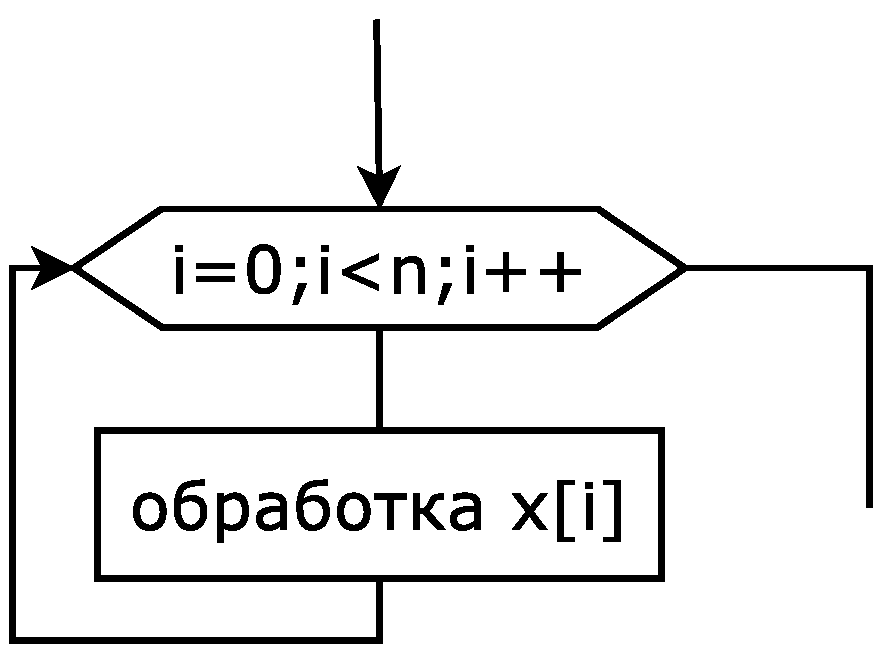
\includegraphics[width=0.3\textwidth]{img/ris_5_1}
\caption{Алгоритм обработки элементов массива}
\label{ch05:refDrawing0}
\end{center}
\end{figure}

Алгоритмы, с помощью которых обрабатывают одномерные массивы, похожи на обработку последовательностей (вычисление суммы,
произведения, поиск элементов по определённому признаку, выборки и т. д.). Отличие заключается в том, что в массиве
одновременно доступны все его компоненты, поэтому становится возможной, например, сортировка его элементов и другие,
более сложные преобразования.

\subsection[Ввод-вывод элементов массива]{Ввод-вывод элементов массива}
Ввод и вывод массивов также осуществляется поэлементно. Блок-схемы алгоритмов ввода и вывода элементов массива
\Sys{X[N]} изображены на рис.~\ref{ch05:refDrawing1}--\ref{ch05:refDrawing2}.

Рассмотрим несколько вариантов ввода массива:
\begin{lstlisting}
//`Вариант 1. Ввод массива с помощью функции \Sys{scanf}.`
//`При организации ввода используются специальные символы: табуляция --- {\textbackslash}t` 
//`и переход на новую строку --- {\textbackslash}n.`
#include <stdio.h>
int main()
{
float x[10]; int i,n; 
printf("\n N="); scanf("%d",&n); //`Ввод размерности массива.`
printf("\n `\Sys{Введите элементы массива}` X \n"); 
for(i=0;i<n;i++)
scanf("%f",x+i);//`Ввод элементов массива в цикле.` 
                //`Обратите внимание, $x+i$ --- адрес $i$-го элемента  массива.`
return 0;
}
\end{lstlisting}

\begin{figure}[htb]
\begin{center}
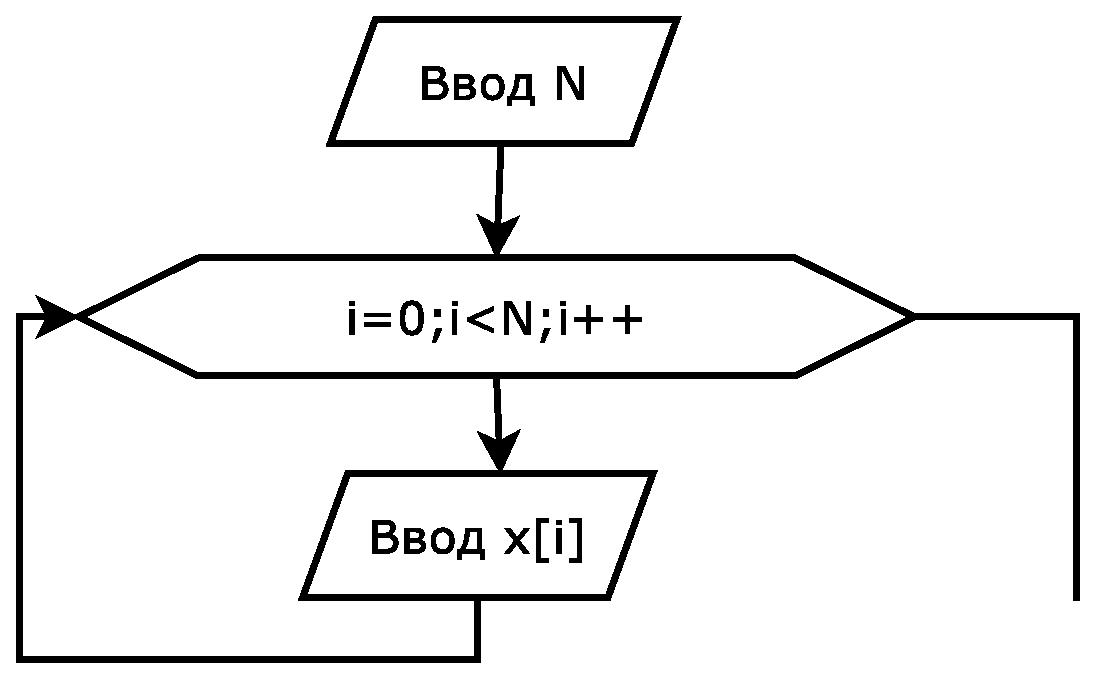
\includegraphics[width=0.4\textwidth]{img/ris_5_2}
\caption{Алгоритм ввода массива \Sys{X[N]}}
\label{ch05:refDrawing1}
\end{center}
\end{figure}

Результат работы программы:
\begin{verbatim}
N=3
Введите элементы массива X 
1.2
-3.8
0.49
\end{verbatim}
\begin{figure}[htb]
\begin{center}
\includegraphics[width=0.4\textwidth]{img/ris_5_3}
\caption{Алгоритм вывода массива \Sys{X[N]}}
\label{ch05:refDrawing2}
\end{center}
\end{figure}

\begin{lstlisting}
//`Вариант 2. Ввод массива с помощью функции \Sys{scanf} и вспомогательной переменной $b$.`
#include <stdio.h>
int main()
{
float x[10],b; int i,n; 
printf("\n N="); scanf("%d",&n); //`Ввод размерности массива.`
printf("\n `Массив` X \n"); 
for(i=0;i<n;i++) 
{ 
  printf("\n `Элемент` %d \t",i); //`Сообщение о вводе элемента.`
  scanf("%f",&b);     //`Ввод переменной $b$.`
  x[i]=b; //`Присваивание элементу массива значения переменной $b$`.
} 
return 0;
}
\end{lstlisting}

Результат работы программы:
\begin{verbatim}
N=4 
Массив X 
Элемент 0 	8.7 
Элемент 1 	0.74 
Элемент 2 	-9 
Элемент 3 	78 
\end{verbatim}

\begin{lstlisting}
//`Вариант 3. Ввод динамического массива с помощью \Sys{cin}.`
#include <iostream>
using namespace std;
int main()
{
  int *X,N,i;
  cout<<"\n N="; cin>>N; //`Ввод размерности массива.`
  X=new int [N]; //`Выделение памяти для динамического массива из $N$ элементов.`
  for (i=0;i<N;i++)
  {
    cout<<"\n X["<<i<<"]="; //`Сообщение о вводе элемента.`
    cin>>X[i];              //`Ввод элементов массива в цикле.`
  }
  delete [] X;
  return 0;
}
\end{lstlisting}

Результат работы программы:
\begin{verbatim}
N=4 
X[0]=1 
X[1]=2 
X[2]=4 
X[3]=5 
\end{verbatim}

Вывод статического или динамического массива можно осуществить несколькими способами:

\begin{lstlisting}
//`Вариант 1. Вывод массива в виде строки.`
for(i=0;i<n;i++) printf("%f \t",X[i]);
//`Вариант 2. Вывод массива в виде столбца.`
for(i=0;i<n;i++) printf("\n %f ",X[i]);
//`Вариант 3. Вывод массива в виде строки.`
for (i=0;i<N;i++) cout <<"\t X["<<i<<"]="<<X[i];
//`Вариант 4. Вывод массива в виде столбца.`
for (i=0;i<N;i++) cout <<"\n X["<<i<<"]="<<X[i];
\end{lstlisting}

\subsection[Вычисление суммы элементов массива]{Вычисление суммы элементов массива}
Дан массив $X$, состоящий из $N$ элементов. Найти сумму элементов этого массива.
Процесс накапливания суммы элементов массива достаточно прост и практически\index{Алгоритм!Сумма элементов массива}
ничем не отличается от суммирования значений некоторой числовой последовательности. Переменной $S$
присваивается значение, равное нулю, затем к переменной $S$ последовательно добавляются элементы
 массива $X$. Блок-схема
алгоритма расчёта суммы приведена на рис.~\ref{ch05:refDrawing3}.

\begin{figure}[htb]
\begin{center}
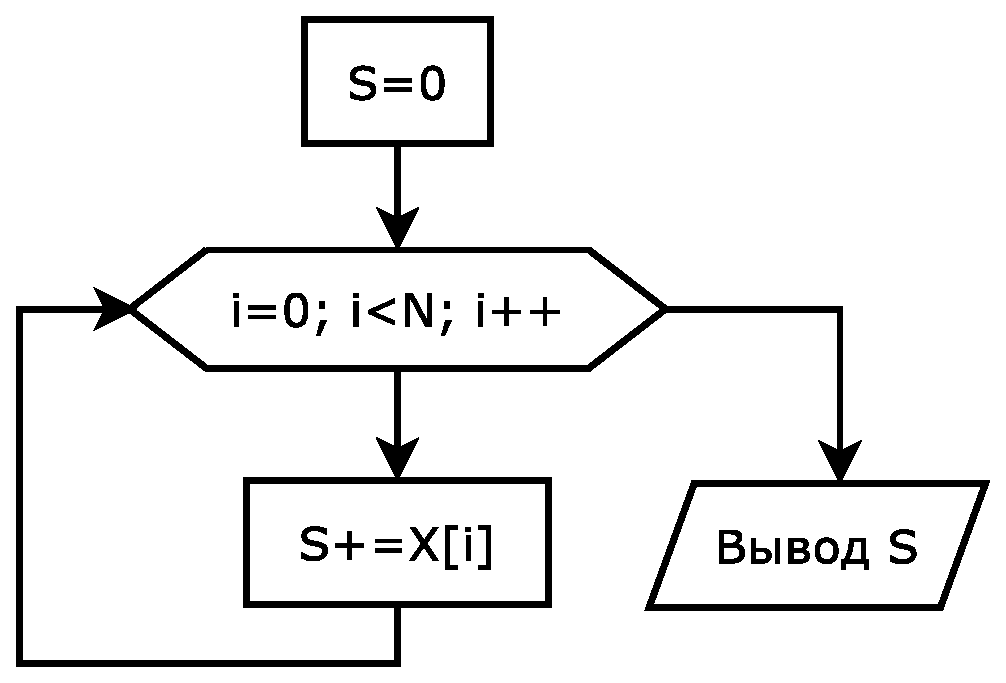
\includegraphics[width=0.4\textwidth]{img/ris_5_4}
\caption{Алгоритм вычисления суммы элементов массива}
\label{ch05:refDrawing3}
\end{center}
\end{figure}

Соответствующий алгоритму фрагмент программы будет иметь вид:
\begin{lstlisting}
for (S=i=0;i<N;i++)
    S+=X[i];
cout<<"S="<<S<<"\n";
\end{lstlisting}

\subsection[Вычисление произведения элементов массива]{Вычисление произведения элементов массива}
Дан массив $X$, состоящий из $N$ элементов. Найти \index{Алгоритм!Произведение
элементов массива}произведение элементов этого массива. Решение этой задачи сводится к тому, что значение переменной
$P$, в которую предварительно была записана единица, последовательно умножается на значение
$i$–го элемента массива. Блок-схема алгоритма приведена на рис.~\ref{ch05:refDrawing4}.

Соответствующий фрагмент программы будет иметь вид:
\begin{lstlisting}
for (P=1,i=0;i<N;i++)
    P*=X[i];
cout<<"P="<<P<<"\n";
\end{lstlisting}

\prg{Задан массив целых чисел. Найти сумму простых чисел и
произведение отрицательных элементов массива.}{gl05:prg0}

Алгоритм решения задачи состоит из следующих этапов.

\begin{enumerate}
\item Вводим массив $X[N]$.
\item Для вычисления суммы в переменную $S$ записываем значение 0, для вычисления произведения в
переменную $P$ записываем 1.
\item В цикле ($i$ изменяется от 0 до $N$-1 с шагом 1) перебираем все элементы
массива $X$, если очередной элемент массива является простым числом, добавляем его к сумме, а если
очередной элемент массива отрицателен, то умножаем его на $P$.
\item Выводим на экран значение суммы и произведения.
\end{enumerate}

\begin{figure}[htb]
\begin{center}
\includegraphics[width=0.4\textwidth]{img/ris_5_5}
\caption{Вычисление произведения элементов массива}
\label{ch05:refDrawing4}
\end{center}
\end{figure}

Блок-схема решения задачи представлена на рис.~\ref{ch05:refDrawing5}. 
Для решения задачи применим функцию (\Sys{prostoe})
проверки, является ли число простым. Текст программы с подробными комментариями приведён далее.
\begin{lstlisting}
#include <iostream>
using namespace std;
//`Текст функции \Sys{prostoe}.`
bool prostoe (int N)
{
    int i;
    bool pr;
    if (N<2) pr=false;
    else
    for(pr=true,i=2;i<=N/2;i++)
        if (N%i==0)
        {
            pr=false;
            break;
        }
    return pr;
}
int main()
{
  int *X,i,N,S,P;
  cout<<"`\Sys{Введите размер массива}` ";cin>>N; //`Ввод размерности массива.`
  X=new int [N]; //`Выделение памяти для хранения динамического массива $X$.`
  cout<<"`\Sys{Ведите массив}` X\n"; //`Ввод массива $X$.`
  for(i=0;i<N;i++)
    {cout<<"X("<<i<<")=";cin>>X[i];}
  for(P=1,S=i=0;i<N;i++) //`В цикле перебираем все элементы массива`
  {
    //`Если очередной элемент массива --- простое число, добавляем его к сумме.`
    if (prostoe(X[i])) S+=X[i];
    //`Если очередной элемент массива отрицателен, умножаем его на P.`
    if (X[i]<0) P*=X[i];
  }
  cout << "S=" <<S<<"\tP="<<P<< endl; //`Вывод S и P на экран.`
  delete [] X; //`Освобождение занимаемой массивом X памяти.`
  return 0;
}
\end{lstlisting}

\begin{figure}[h]
\begin{center}
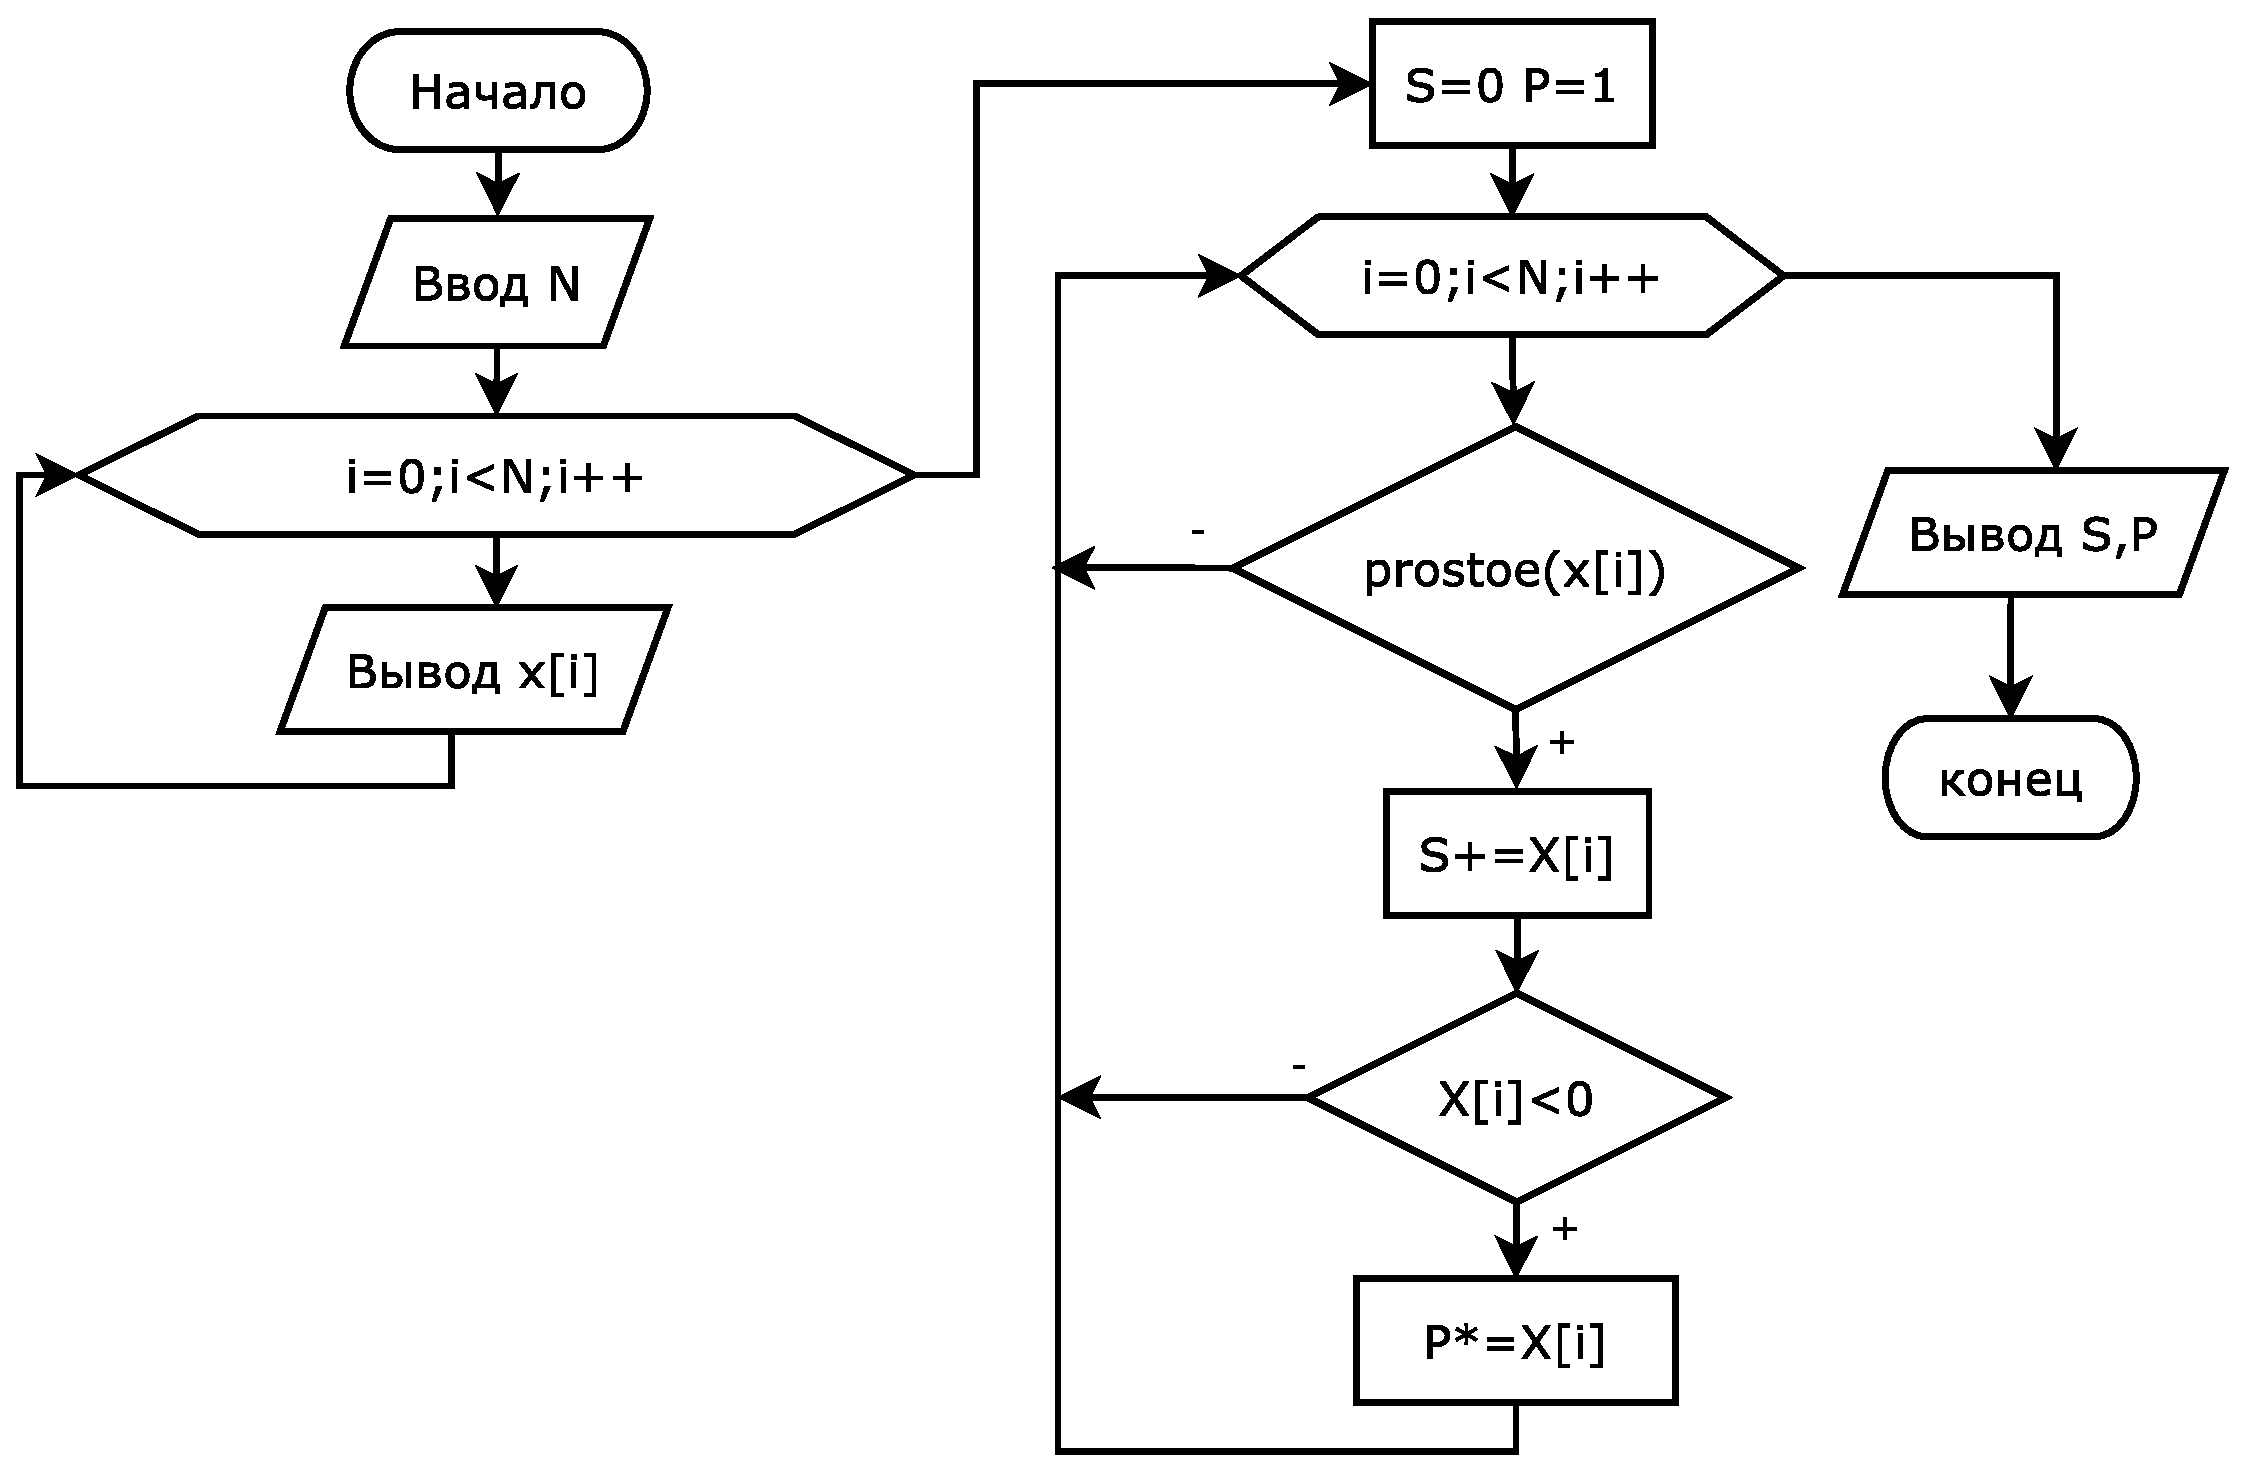
\includegraphics[width=0.7\textwidth]{img/ris_5_6}
\caption{Блок-схема алгоритма решения задачи~\ref{gl05:prg0}}
\label{ch05:refDrawing5}
\end{center}
\end{figure}

Результаты работы программы представлены ниже.
\begin{verbatim}
Введите размер массива 10 
Ведите массив Х 
X(0)=-7 
X(1)=-9 
X(2)=5 
X(3)=7 
X(4)=2 
X(5)=4 
X(6)=6 
X(7)=8 
X(8)=10 
X(9)=12 
S=14	P=63 
\end{verbatim}

\prg{Дан массив $A$, состоящий из $k$ целых положительных чисел. 
Записать все чётные по значению элементы массива $A$ в массив $B$.}{gl05:prg0a}

На рис.~\ref{ch05:refDrawing6a} представлен фрагмент алгоритма решения данной задачи. 
Здесь индексы массива $A$ хранятся в переменной $i$, а для номеров массива $B$ 
зарезервирована переменная $m$. Операция, выполняемая в блоке 1, означает, 
что в массиве $A$ может не быть искомых элементов. Далее организован цикл (блок 2), 
с помощью которого можно обращаться к элементам массива $A$. Если условие в блоке 3 
выполняется, то переменная $m$ увеличивается на единицу, а значение соответствующего 
элемента массива $A$ записывается в массив В под номером $m$ (блок 4). Условный блок 5 
необходим для того, чтобы проверить, выполнилось ли хотя бы раз условие поиска (блок 2). 
Если массив $B$ сформирован, то он выводится на экран (блоки 6, 7), в противном случае 
выдаётся соответствующее сообщение (блок 8).

\begin{figure}[h]
\begin{center}
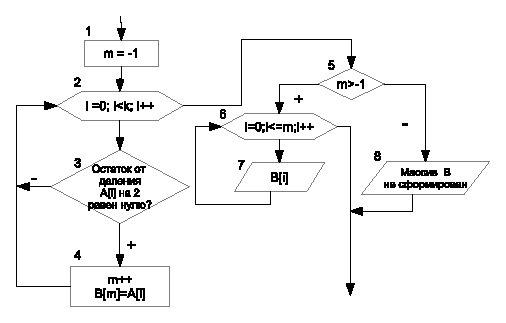
\includegraphics[width=0.7\textwidth]{img/ris_5_7a}
\caption{Алгоритм решения задачи~\ref{gl05:prg0a}}
\label{ch05:refDrawing6a}
\end{center}
\end{figure}

Приведённый ниже фрагмент программы реализует описанный алгоритм:
\begin{lstlisting}
for (m=-1,i=0; i<k; i++)
{
  if (A[i]%2==0) //`Если элемент чётный, то`
  {
    m++;         //`увеличить значение индекса массива В` 
    B[m]=A[i];   //`и записать элемент в массив В.`
  }
}
if (m>-1) //`Если чётные элементы найдены, то распечатать сформированный массив.`
  for (i=0;i<=m;cout<<B[i]<<"\t",i++);
else //`иначе, выдать сообщение,`
  cout<<"`\Sys{Массив $B$ не сформирован!}`"<<endl; 
\end{lstlisting}

\subsection[Поиск максимального элемента в массиве и его номера]{Поиск максимального элемента в массиве и его номера}
Дан массив \Sys{X}, состоящий из \Sys{n} элементов. Найти \index{Алгоритм!Поиск максимального
(минимального) элемента массива и номера}максимальный элемент массива и номер, под которым он хранится в массиве. 

Алгоритм решения задачи следующий. Пусть в переменной с именем \Sys{Max} хранится значение максимального
элемента массива, а в переменной с именем \Sys{Nmax}~– его номер. Предположим, что нулевой элемент массива
является максимальным, и запишем его в переменную \Sys{Max}, а в \Sys{Nmax} --- его номер (то
есть ноль). Затем все элементы, начиная с первого, сравниваем в цикле с максимальным. Если текущий элемент массива
оказывается больше максимального, то записываем его в переменную \Sys{Max}, а в переменную
\Sys{Nmax}~– текущее значение индекса \Sys{i}. Процесс определения максимального элемента в
массиве приведён в таблице \ref{ch05:refTable2} и изображён при помощи блок-схемы на рис. \ref{ch05:refDrawing6}.
Соответствующий фрагмент программы имеет вид:
\begin{lstlisting}
for (Max=X[0],Nmax=i=0;i<n;i++)
  if (Max<X[i])
  {
    Max=X[i];
    Nmax=i;
  }
cout<<"Max="<<Max<<"\n";
cout<<"Nmax="<<Nmax<<"\n";
\end{lstlisting}

{%\tabcolsep=0.5em
\noindent\small
\begin{longtable}{|p{0.4\textwidth}|c|c|c|c|c|c|}
\caption{Определение максимального элемента и его номера в массиве} \label{ch05:refTable2}\\
\hline
\endfirsthead
\multicolumn{7}{c}%
{{\tablename\ \thetable{} --- продолжение}} \\
\hline
\endhead
Номера элементов &0 &1 &2 &3 &4 &5\\\hline
Исходный массив &4 &7 &3 &8 &9 &2\\\hline
Значение переменной $Max$  &4 &7 &7 &8 &9 &9\\\hline
Значение переменной $Nmax$ &1 &2 &2 &4 &5 &5\\\hline
\end{longtable}
}

\begin{figure}[htb]
\begin{center}
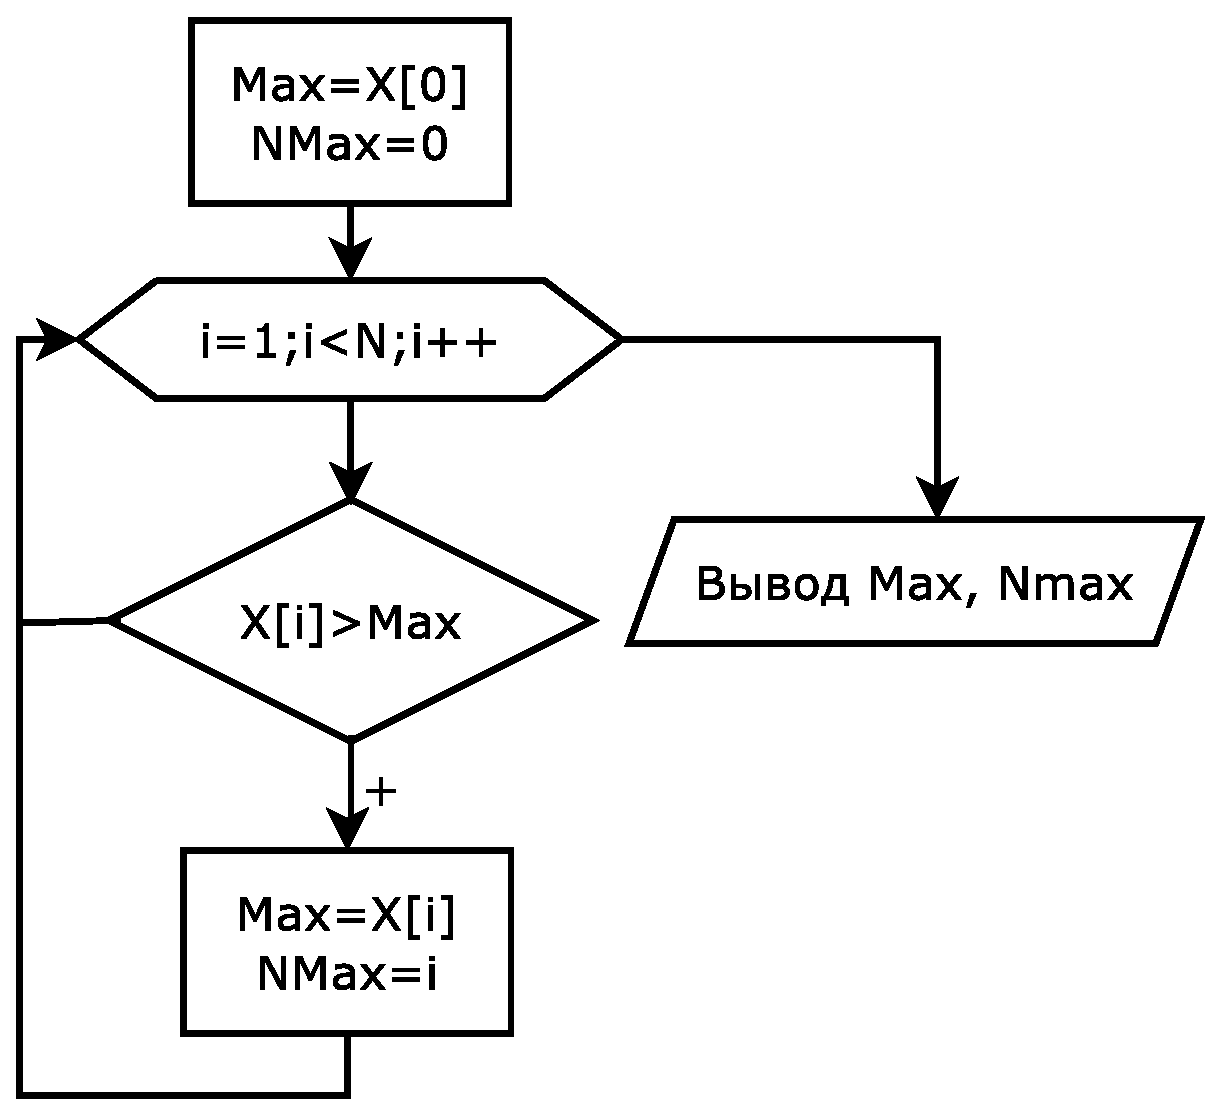
\includegraphics[width=0.4\textwidth]{img/ris_5_7}
\caption{Поиск максимального элемента и его номера в массиве}
\label{ch05:refDrawing6}
\end{center}
\end{figure}




При поиске максимального элемента и его номера, можно найти только номер максимального элемента, а потом по номеру извлечь
значение максимального элемента из массива.

Текст программы поиска номера максимального элемента:
\begin{lstlisting}
#include <iostream>
using namespace std;
int main()
{
  float *X;
  int i,N,nom;
  cout<<"`Введите размер массива` ";cin>>N; //`Ввод размерности динамического массива`
  X=new float[N]; //`Выделение памяти для хранения динамического массива $X$.`
  cout<<"`\Sys{Введите элементы массива}` X\n"; //`Ввод динамического массива $X$.`
  for(i=0;i<N;i++)
    cin>>X[i];
  //`В переменной $nom$ будем хранить номер максимального элемента.` 
  nom=0; //`Предположим, что максимальным элементом является элемент с номером 0.`
  for(i=1;i<N;i++)
  //`Если очередной элемент больше X[nom], значит nom не является номером максимального`
  //`элемента, элемент с номером $i$ больше элемента X[nom], поэтому переписываем`
  //`число i в переменную nom.`
    if (X[i]>X[nom]) nom=i;
  cout << "`\Sys{Максимальный элемент}`="<<X[nom]<<", `его номер`=" << nom << endl;
  return 0;
}
\end{lstlisting}

\Emph{Совет.} Алгоритм поиска минимального элемента в массиве будет отличаться от приведённого выше лишь тем, что в
условном блоке и, соответственно, в конструкции \Sys{if} текста программы знак поменяется с <<{<}>> на <<{>}>>.

Рассмотрим несколько задач.

\prg{Найти минимальное простое число в целочисленном массиве
x[N].}{gl05:prg1}

Эта задача относится к классу задач поиска минимума (максимума) среди элементов, удовлетворяющих условию. Подобные
задачи рассматривались в задачах на обработку последовательности чисел. Здесь поступим аналогично. Блок-схема приведена
на рис.~\ref{ch05:refDrawing7}.

Необходимо первое простое число объявить минимумом, а все последующие простые элементы массива сравнивать с минимумом.
Будем в цикле последовательно проверять, является ли элемент массива простым числом (функция
\Sys{prostoe}). Если \Sys{X[i]} является простым числом, то количество простых чисел
(\Sys{k}) увеличиваем на 1 (\Sys{k++}), далее, проверяем, если\Sys{ k} равен 1
(\Sys{if (k==1)}), то этот элемент объявляем минимальным (\Sys{min=x[i]; nom=i;}), иначе
сравниваем его с минимальным (\Sys{if (x[i]<min) \{min=x[i];nom=i;\}}).

Текст программы:
\begin{lstlisting}
#include <iostream>
using namespace std;
bool prostoe (int N)
{ int i;  bool pr;
  if (N<2) pr=false;
  else
  for(pr=true,i=2;i<=N/2;i++)
    if (N%i==0)
    {
       pr=false;
       break;
    }
  return pr;
}
int main(int argc, char **argv)
{
  int i,k,n,nom,min,*x;
  cout<<"n="; cin>>n; //`Ввод количества элементов в массиве.`
  x=new int [n]; //`Выделяем память для динамического массива x.`
  cout<<"`\Sys{Введите элементы массива}` X"; //`Ввод элементов массива.`
  for(i=0;i<n;i++)
    cin>>x[i];
  //`С помощью цикла по переменной $i$, перебираем все элементы в массиве $x$,` 
  //`$k$ --- количество простых чисел в массиве.`
  for(i=k=0;i<n;i++)
  //`Проверяем, является ли очередной элемент массива простым числом.` 
    if (prostoe(x[i])) //`Если \Sys{x[i]} --- простое число.`
    {
      k++; //`Увеличиваем счётчик количества простых чисел в массиве.`
      //`Если текущий элемент является первым простым числом в массиве,`
      // `объявляем его минимумом, а его номер сохраняем в перемнной nom.`
      if (k==1) {min=x[i];nom=i;}
    else
    //`Все последующие простые числа в массиве сравниваем с минимальным простым числом.`
    //`Если текущее число меньше \Sys{min}, перезаписываем его в переменную \Sys{min},`
    //`а его номер --- в переменную \Sys{nom}.`
      if (x[i]<min) {min=x[i];nom=i;}
    }
//`Если в массиве были простые числа, выводим значение и номер минимального простого числа.`
  if (k>0)
    cout<<"min="<<min<<"\tnom="<<nom<<endl;
  //`Иначе выводим сообщение о том, что в массиве нет простых чисел.`
  else cout<<"`\Sys{Нет простых чисел в массиве}`"<<endl;
  return 0;
}
\end{lstlisting}


\begin{figure}[htb]
\begin{center}
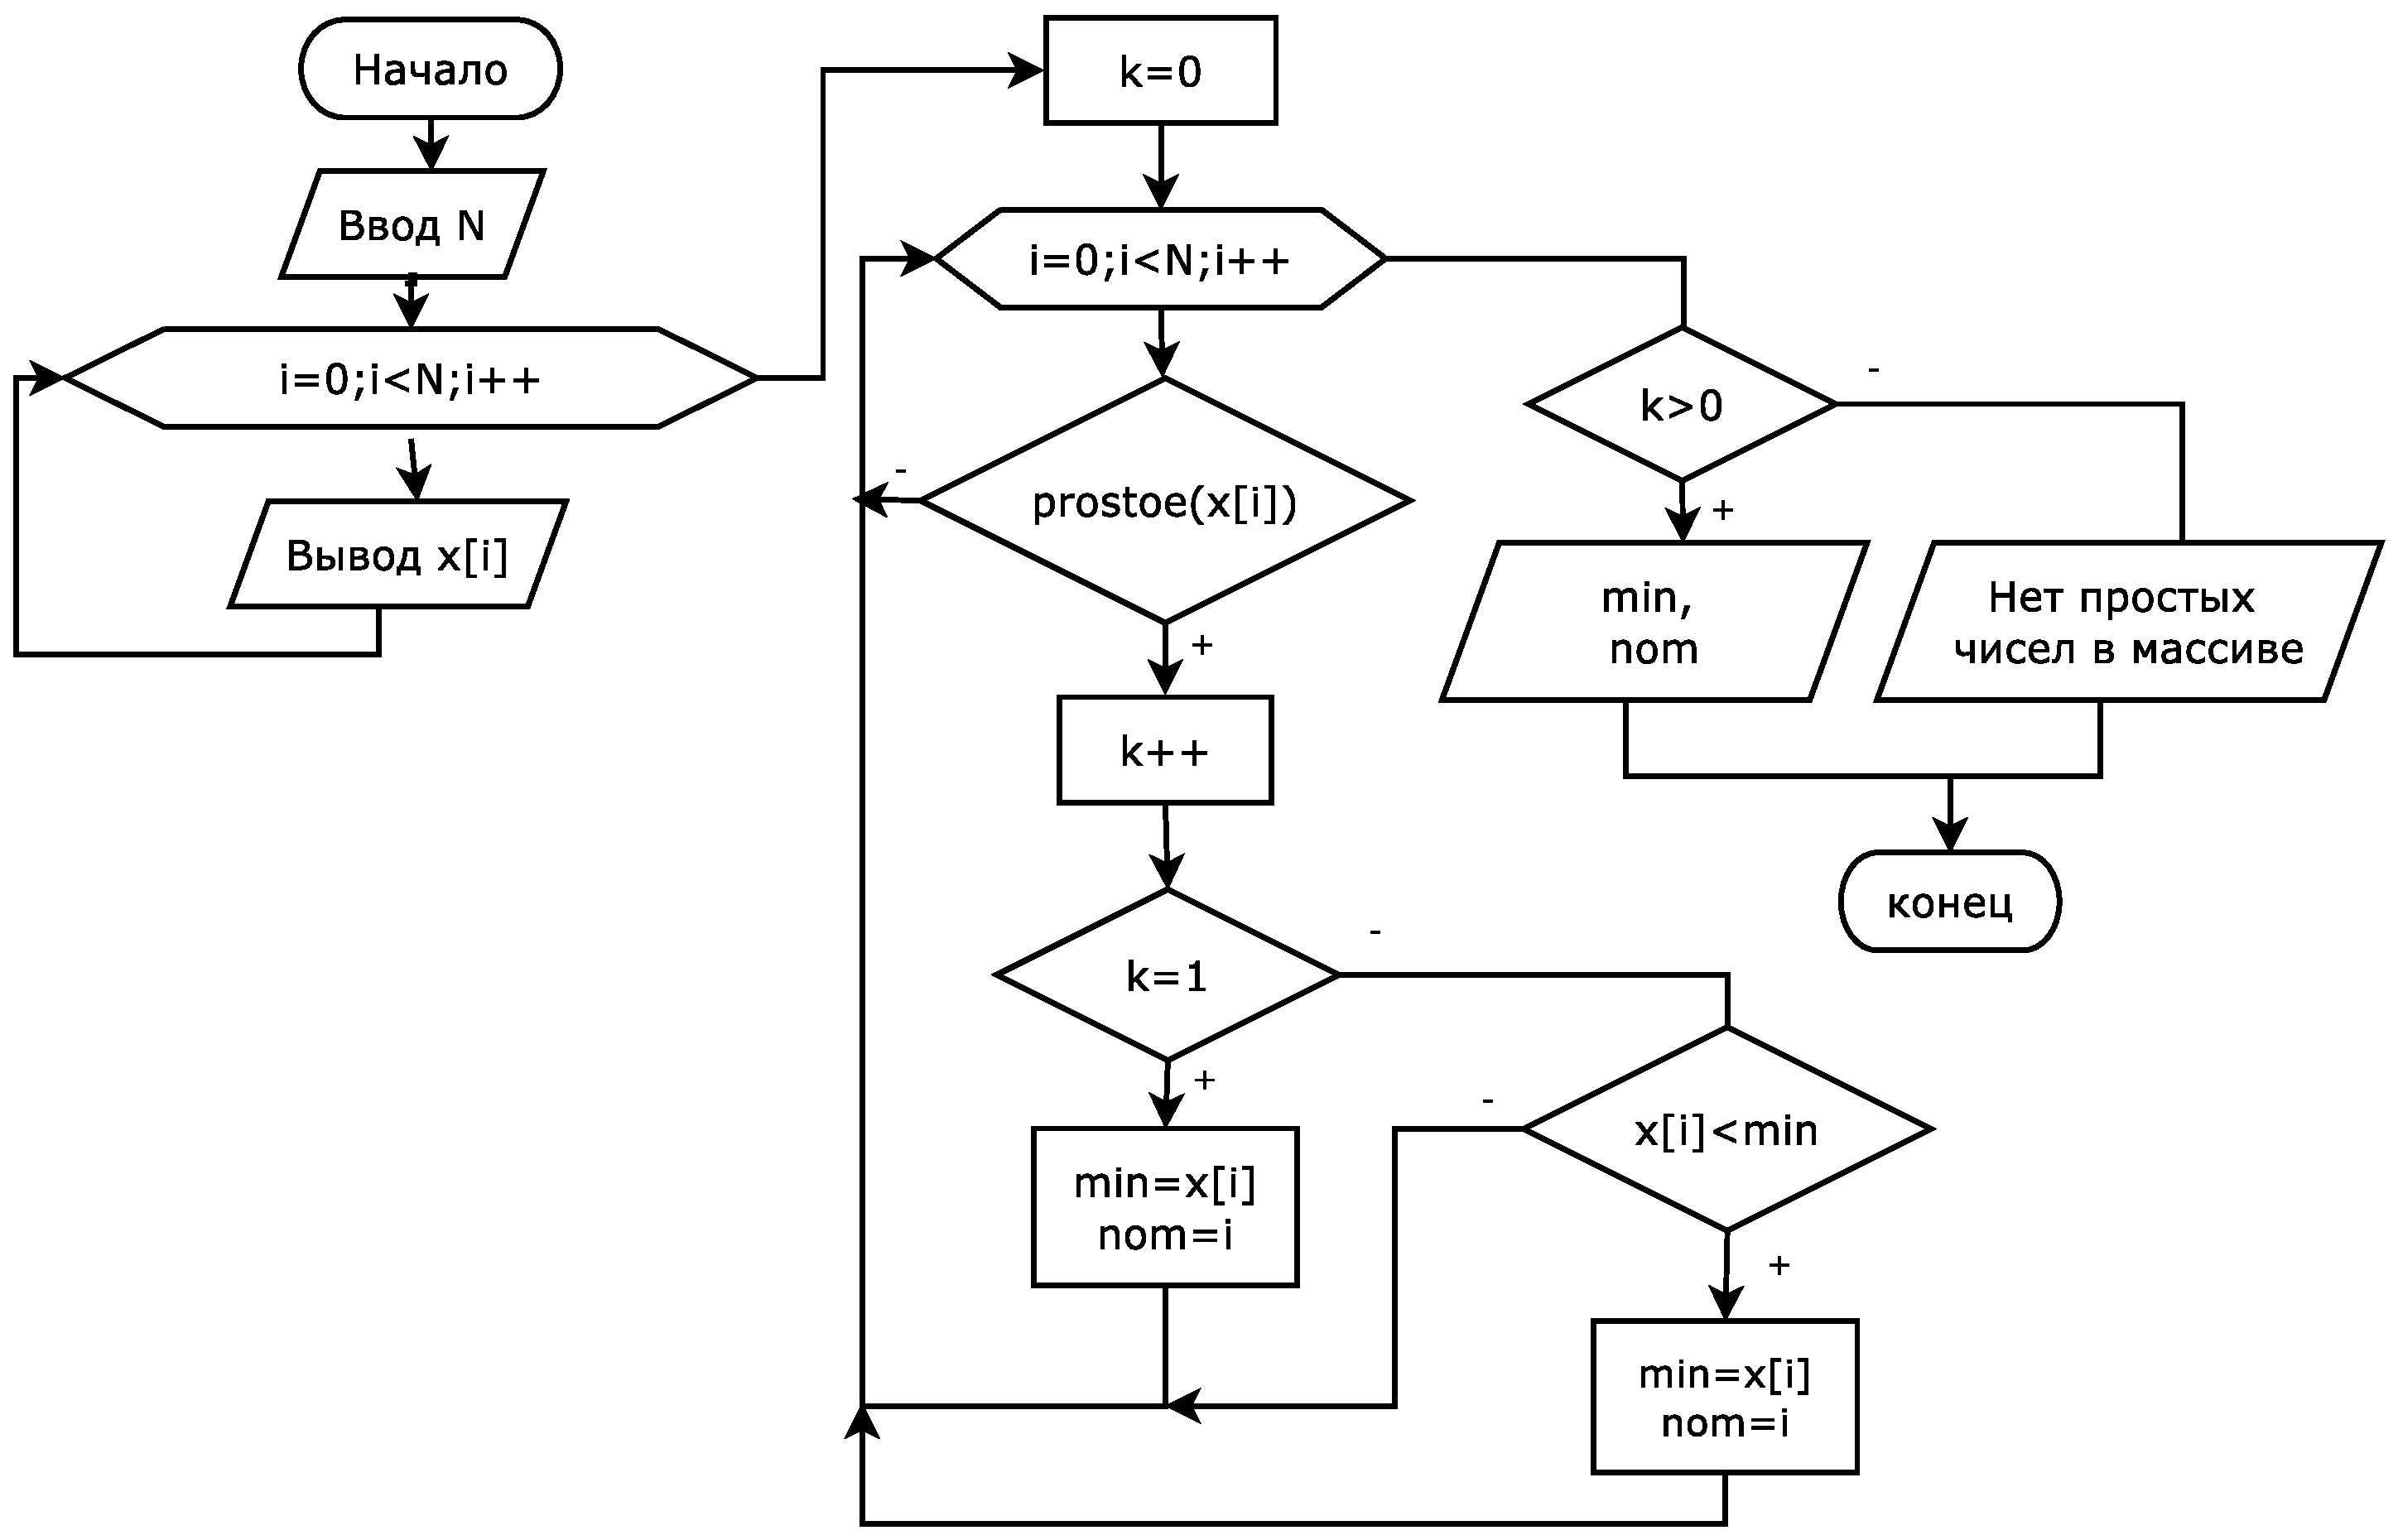
\includegraphics[width=0.8\textwidth]{img/ris_5_8}
\caption{Блок-схема решения задачи~\ref{gl05:prg1}}
\label{ch05:refDrawing7}
\end{center}
\end{figure}



Аналогичным образом можно написать программу любой задачи поиска минимума (максимума) среди элементов, удовлетворяющих
какому-либо условию (минимум среди положительных элементов, среди чётных и т.д.). 

\prg{Найти $k$ минимальных чисел в вещественном массиве.}{gl05:prg2}

Перед решением этой довольно сложной задачи рассмотрим более простую задачу.

Найти два наименьших элемента в массиве. Фактически надо найти номера
(\Sys{nmin1}, \Sys{nmin2}) двух наименьших элементов
массива. На первом этапе надо найти номер минимального (\Sys{nmin1}) элемента массива. На втором этапе
надо искать номер минимального элемента, при условии, что он не равен \Sys{nmin1}. Вторая часть очень
похожа на предыдущую задачу (минимум среди элементов, удовлетворяющих условию, в этом случае условие имеет вид
\Sys{i!=nmin1}).

Решение задачи с комментариями:

\begin{lstlisting}
#include <iostream>
using namespace std;
int main(int argc, char **argv)
{
  int kvo,i,n,nmin1,nmin2;
  double *X;
  cout<<"n=";cin>>n;
  X=new double [n];
  cout<<"`Введите элементы массива` X\n";
  for(i=0;i<n;i++)
    cin>>X[i];
  //`Стандартный алгоритм поиска номера первого минимального элемента (\Sys{nmin1}).`
  for(nmin1=0,i=1;i<n;i++)
    if (X[i]<X[nmin1]) nmin1=i;
  //`Второй этап --- поиск номера минимального элемента среди элементов, номер` 
  //`которых не совпадает \Sys{nmin1}. \Sys{kvo} --- количество таких элементов.`
  for(kvo=i=0;i<n;i++)
    if (i!=nmin1) //`Если номер текущего элемента не совпадает с nmin1`, 
    {
      kvo++; //`увеличиваем количество таких элементов на 1.`
      //`Номер первого элемента, индекс которого не равен \Sys{nmin1},` 
      //`объявляем номером второго минимального элемента.`
      if (kvo==1) nmin2=i; 
      else
      //`очередной элемент, индекс которого не равен \Sys{nmin1}, сравниваем с минимальным,` 
      //`если он меньше, номер перезаписываем в переменную \Sys{nmin2}.`
      if (X[i]<X[nmin2]) nmin2=i;
    }
  //`Вывод двух минимальных элементов и их индексов.`
  cout<<"nmin1="<<nmin1<<"\tmin1="<<X[nmin1]<<endl;
  cout<<"nmin2="<<nmin2<<"\tmin2="<<X[nmin2]<<endl;
  return 0;
}
\end{lstlisting}


По образу и подобию этой задачи можно написать задачу поиска трёх минимальных элементов в массиве. Первые два этапа
(поиск номеров двух минимальных элементов в массиве) будут полным повторением кода, приведённого выше. На третьем этапе
нужен цикл, в котором будем искать номер минимального элемента, при условии, что его номер не равен
\Sys{nmin1} и \Sys{nmin2}. Авторы настоятельно рекомендуют читателям самостоятельно написать
подобную программу. Аналогично можно написать программу поиска четырёх минимальных элементов. Однако при этом
усложняется и увеличивается код программы. К тому же, рассмотренный приём не позволит решить задачу в общем случае
(найти \Sys{k} минимумов). 

Для поиска $k$ минимумов в массиве можно поступить следующим образом. Будем формировать массив
\Sys{nmin}, в котором будут храниться номера минимальных элементов массива \Sys{x}. Для его
формирования организуем цикл по переменной $j$ от 0 до \Sys{k-1}. При
каждом вхождении в цикл в массиве \Sys{nmin} элементов будет \Sys{j-1} элементов,i и мы будем
искать $j$-й минимум (формировать $j$-й элемент массива). Алгоритм формирования
$j$-го элемента состоит в следующем: необходимо найти номер минимального элемента в массиве \Sys{x},
исключая номера, которые уже хранятся в массиве \Sys{nmin}. Внутри цикла по $j$
необходимо выполнить такие действия. Для каждого элемента массива \Sys{x} (цикл по переменной
$i)$ проверить содержится ли номер в массиве \Sys{nmin}, если не содержится, то
количество (переменная \Sys{kvo}) таких элементов увеличить на $1$. Далее, если
\Sys{kvo} равно $1$, то это первый элемент, который не содержится в массиве
\Sys{nmin}, его номер объявляем номером минимального элемента массива (\Sys{nmin\_temp=i;}).
Если \Sys{kvo>1}, сравниваем текущий элемент
\Sys{x[i]} с минимальным (\Sys{if (x[i]<X[nmin\_temp]) nmin\_temp=i;}).
Блок-схема алгоритма поиска $k$ минимальных элементов массива представлена на рис.~\ref{ch05:refDrawing8}\footnote{В
блок-схеме отсутствует ввод данных и вывод результатов.}.  Далее приведён текст программы с комментариями.
\begin{lstlisting}
#include <iostream>
using namespace std;
int main(int argc, char **argv)
{
  int p,j,i,n,*nmin,k,kvo,nmin_temp;
  bool pr;
  double *x;
  cout<<"n=";cin>>n;
  x=new double [n];
  cout<<"`Введите элементы массива Х`\n";
  for(i=0;i<n;i++)
    cin>>x[i];
  cout<<"`Введите количество минимумов`\n";cin>>k;
  nmin=new int[k];
  for(j=0;j<k;j++) //`Цикл по переменной $j$ для поиска номера $j+1$ минимального элемента`
  {
    kvo=0;
    for(i=0;i<n;i++) //`Перебираем все элементы массива.`
    {
      //`Цикл по переменной $p$ проверяет, содержится ли номер $i$ в массиве nmin.`
      pr=false;
      for(p=0;p<j;p++)
        if (i==nmin[p]) pr=true;
      if (!pr) //`Если не содержится, то количество элементов увеличить на 1.`
      {
        kvo++;
        //`Если kvo=1, то найден первый элемент, который не содержится в массиве`
        //`nmin, его номер объявляем номером минимального элемента массива`
        if (kvo==1) nmin_temp=i;
        else
          //`Если kvo>1, сравниваем текущий элемент x[i] с минимальным.`
          if (x[i]<x[nmin_temp]) nmin_temp=i;
      }
    }
    nmin[j]=nmin_temp; //`Номер очередного минимального элемента записываем в массив.`		
  }
  for(j=0;j<k;j++) //`Вывод номеров и значений $k$ минимальных элементов массива.`
    cout<<"nmin1="<<nmin[j]<<"\tmin1="<<x[nmin[j]]<<endl;
  return 0;
}
\end{lstlisting}

\begin{figure}[htb]
\begin{center}
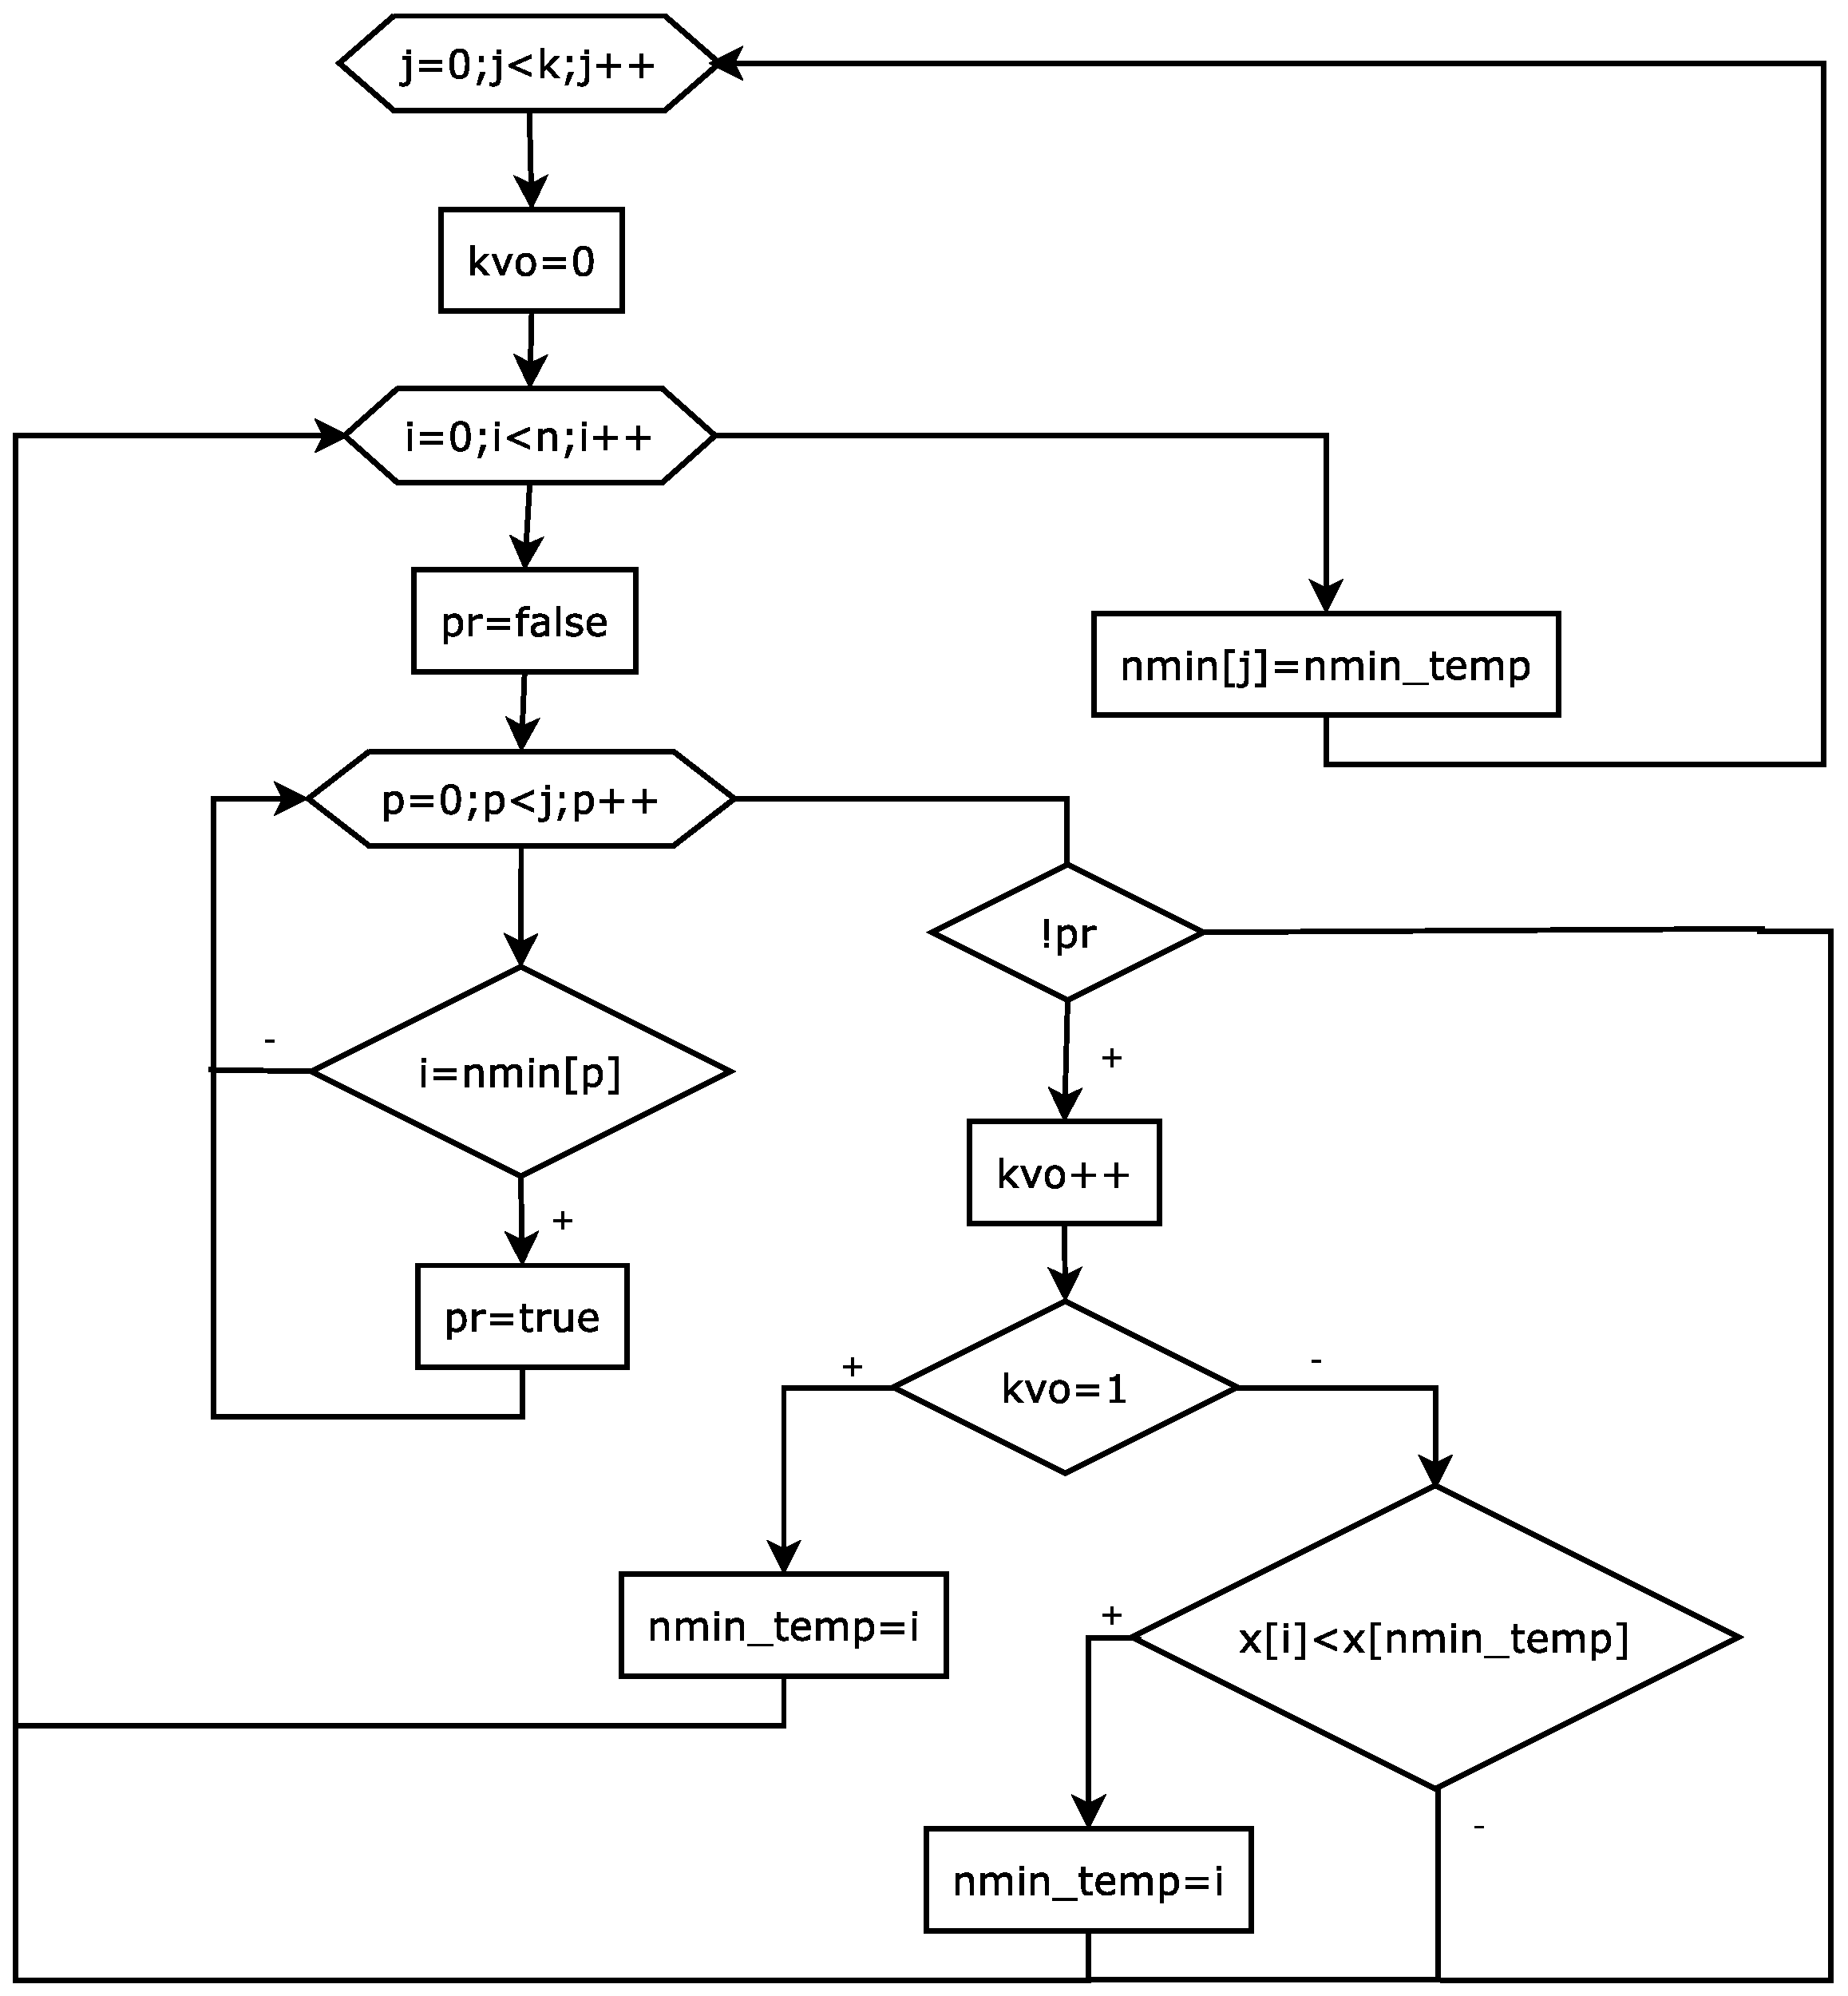
\includegraphics[width=0.7\textwidth]{img/ris_5_9}
\caption{Блок-схема алгоритма поиска $k$ минимальных элементов в массиве $x$.}
\label{ch05:refDrawing8}
\end{center}
\end{figure}

Проверку, содержится ли число \Sys{i} в массиве \Sys{nmin}, можно оформить в виде функции,
тогда программа может быть записана следующим образом:
\begin{lstlisting}
#include <iostream>
using namespace std;
//`Функция проверяет, содержится ли число i в массиве x из n элементов.`
//`Функция возвращает true, если содержится, и false, если не содержится.`
bool proverka(int i, int *x, int n)
{
  bool pr;
  int p;
  pr=false;
  for(p=0;p<n;p++)
    if (i==x[p]) pr=true;
  return pr;
}
int main(int argc, char **argv)
{
  int  j,i,n,*nmin,k,kvo,nmin_temp;
  double *x;
  cout<<"n=";cin>>n;
  x=new double [n];
  cout<<"`\Sys{Введите элементы массива Х}`\n";
  for(i=0;i<n;i++)
    cin>>x[i];
  cout<<"`\Sys{Введите количество минимумов}`\n";cin>>k;
  nmin=new int[k];
  for(j=0;j<k;j++) //`Цикл по переменной $j$ для поиска номера $j+1$ минимального элемента`
  {
    kvo=0;
    for(i=0;i<n;i++) //`Перебираем все элементы массива.`
    {
    //`Вызов функции proverka, определяем, содержится ли число $i$ в массиве nmin из $j$ элементов`
      if (!proverka(i,nmin,j)) 
      {
        kvo++;
        if (kvo==1) nmin_temp=i;
        else
          if (x[i]<x[nmin_temp]) nmin_temp=i;
      }
    }
    nmin[j]=nmin_temp;		
  }
  for(j=0;j<k;j++) //`Вывод номеров и значений k минимальных элементов массива.`
    cout<<"nmin1="<<nmin[j]<<"\tmin1="<<x[nmin[j]]<<endl;
  return 0;
}
\end{lstlisting}


Авторы настоятельно рекомендуют читателю разобрать все версии решения задачи~\ref{gl05:prg2}.

\prg{Поменять местами максимальный и минимальный элементы в массиве X.}{gl05:prg3}

Алгоритм решения задачи можно разбить на следующие этапы.

\begin{enumerate}
\item Ввод массива.
\item Поиск номеров максимального (\Sys{nmax}) и минимального (\Sys{nmin}) элементов массива.
\item Обмен элементов местами. Не получится записать «в лоб» (\lstinline!X[nmax]=X[nmin];!
\mbox{\lstinline!X[nmin]=X[nmax];!)}. 
При таком присваивании мы сразу же теряем максимальный элемент. 
Поэтому нам понадобится временная (буферная) переменная temp. Обмен элементов
местами должен быть таким:
\mbox{\lstinline!temp=X[nmax]; X[nmax]=X[nmin]; X[nmin]=temp;!}
\end{enumerate}

Далее приведён текст программы с комментариями.
\begin{lstlisting}
#include <iostream>
using namespace std;
int main(int argc, char **argv)
{
  int i,N,nmax,nmin;
  float temp;
  cout<<"N=";cin>>N;
  float X[N];
  cout<<"`\Sys{Введите элементы массива Х}`\n";
  for(i=0;i<N;i++)
    cin>>X[i];
  //`Поиск номеров максимального и минимального элементов массива.`
  for(nmax=nmin=0,i=1;i<N;i++)
  {
    if (X[i]<X[nmin]) nmin=i;
    if (X[i]>X[nmax]) nmax=i;
  }
  //`Обмен максимального и минимального элементов местами.`
  temp=X[nmax];X[nmax]=X[nmin]; X[nmin]=temp;
  cout<<"`Преобразованный массив Х`\n"; //`Вывод преобразованного массива.`
  for(i=0;i<N;i++)
    cout<<X[i]<<" ";
  cout<<endl;
  return 0;
}
\end{lstlisting}

\prg{Найти среднее геометрическое среди простых чисел, расположенных между
максимальным и минимальным элементами массива.}{gl05:prg4}

Среднее геометрическое $k$ элементов ($SG)$ можно вычислить по формуле 
$SG=\sqrt[{k}]{P}$, $P$ --- произведение $k$ элементов. При решении этой задачи
необходимо найти  произведение и количество простых чисел, расположенных между максимальным и минимальным элементами.

Алгоритм решения задачи состоит из следующих этапов:

\begin{enumerate}
\item Ввод массива.
\item Поиск номеров максимального (\Sys{nmax}) и минимального (\Sys{nmin}) элементов массива.
\item В цикле перебираем все элементы массива, расположенные между максимальным и минимальным элементами. Если текущий
элемент является простым числом, то необходимо увеличить количество простых чисел на 1, и умножить $P$ на значение
элемента массива.
\item Вычислить  $SG=\sqrt[{k}]{P}$ .
\end{enumerate}
При решении этой задачи следует учитывать, что неизвестно, какой элемент расположен раньше --- максимальный или минимальный.

Текст программы с комментариями приведён ниже.
\begin{lstlisting}
#include <iostream>
#include <math.h>
using namespace std;
bool prostoe (int N)
{
  int i;
  bool pr;
  if (N<2) pr=false;
  else
    for(pr=true,i=2;i<=N/2;i++)
      if (N%i==0)
      {
         pr=false;
         break;
      }
  return pr;
}
int main(int argc, char **argv)
{
  int i,k,n,nmax,nmin, p, *x;
  cout<<"n="; cin>>n; //`Ввод количества элементов в массиве.`
  x=new int [n]; //`Выделяем память для динамического массива x.`
  cout<<"`Введите элементы массива X`"; //`Ввод элементов массива.`
  for(i=0;i<n;i++)
    cin>>x[i];
  //`Поиск номеров максимального и минимального элементов в массиве.`
  for(nmax=nmin=i=0;i<n;i++)
  {
    if (x[i]<x[nmin]) nmin=i;
    if (x[i]>x[nmax]) nmax=i;
  }
  if (nmin<nmax)
    for(p=1,k=0,i=nmin+1;i<nmax;i++)
    //`\emph{Обратите особое внимание на использование в следующей строке фигурной скобки}` 
    //`\emph{(составного оператора). В цикле всего один оператор!!! При этом, при отсутствии}`
    //`\emph{составного оператора, программа начинает считать с ошибками!!!}`
    {
      //`Проверяем, является ли очередной элемент массива простым числом.`
      if (prostoe(x[i])) //`Если x[i] --- простое число.`
      {
      //`Домножаем y[i] на p, а также увеличиваем счётчик количества простых чисел в массиве.`
        k++;p*=x[i];
      }
    }
  else
    for(p=1,k=0,i=nmax+1;i<nmin;i++)
      //`Проверяем, является ли очередной элемент массива простым числом.`
      if (prostoe(x[i])) //`Если x[i] --- простое число.`
      {//`Домножаем y[i] на p, а также увеличиваем счётчик количества простых чисел в массиве.`
        k++;p*=x[i];
      }
    //`Если в массиве были простые числа, выводим среднее геометрическое этих чисел на экран`
    if (k>0)
      cout<<"SG"<<pow(p,1./k)<<endl;
    //`Иначе выводим сообщение о том, что в массиве нет простых чисел.`
    else cout<<"`Нет простых чисел в массиве`"<<endl;
  return 0;
}
\end{lstlisting}


\subsection[Удаление элемента из массива]{Удаление элемента из массива}
Для \index{Алгоритм!Удаление элемента из массива} удаления элемента с индексом $m$ из массива $X$,
состоящего из $n$ элементов,  нужно записать $(m+1)$-й элемент на место элемента $m$,
$(m+2)$-й --- на место $(m+1)$-го и т.д., $(n-1)$-й --- на место $(n-2)$-го. После удаления количество
элементов в массиве уменьшилось на 1 (рис.~\ref{ch05:refDrawing9}). 

\begin{figure}[htb]
\begin{center}
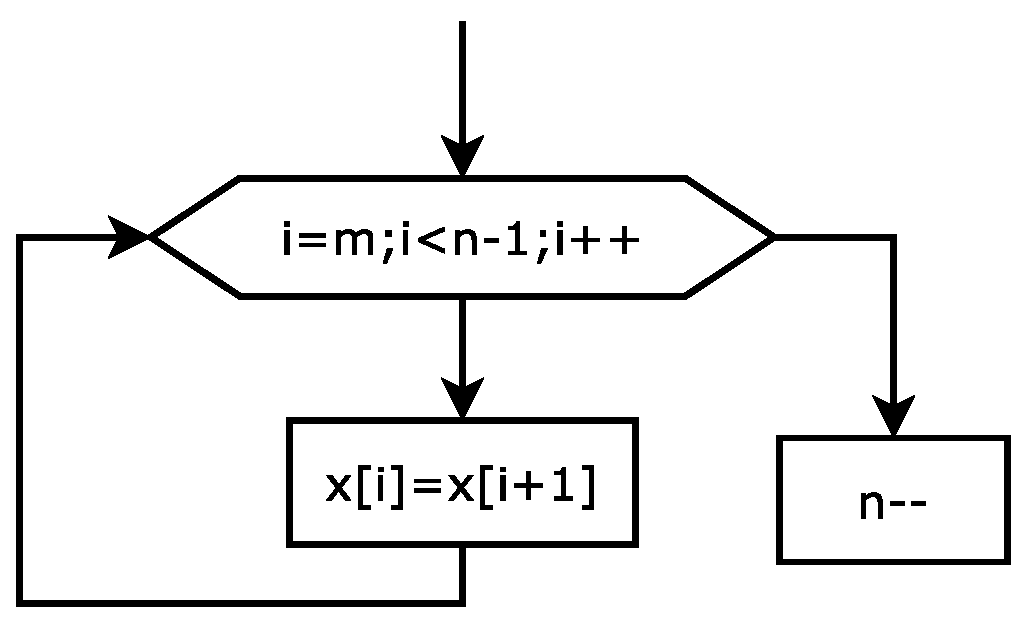
\includegraphics[width=0.4\textwidth]{img/ris_5_10}
\caption{Алгоритм удаления элемента из массива}
\label{ch05:refDrawing9}
\end{center}
\end{figure}

Фрагмент программы на \Sys{С++}:
\begin{lstlisting}
cout<<"\n m="; cin>>m; //`Ввод номера элемента, подлежащего удалению.` 
for (i=m;i<n-1;X[i]=X[i+1],i++); //`Удаление m-го элемента.`
n--;
for (i=0;i<n-1;i++)cout<<X[i]<<"\t"; //`Вывод изменённого массива.`
\end{lstlisting}

При написании программ, в которых удаляются элементы из массива, следует учитывать тот факт, что после удаления элемента
все элементы, расположенные после удалённого, изменяют свои номера (индексы уменьшаются на один). Это особенно важно
при удалении нескольких элементов из массива. Рассмотрим несколько задач.

\prg{Удалить из массива \Sys{x[20]} все элементы с пятого по десятый.}{gl05:prg5}

При решении задач, связанных с удалением подряд идущих элементов, следует понимать, что после удаления очередного
элемента следующий переместился на место удалённого. Поэтому далее нужно будет удалять элемент с тем же самым номером. В
нашем случае подлежит удалению 6 элементов с пятого по десятый. Однако, реально надо будет 6 раз удалить элемент с
номером 5. Блок-схема алгоритма представлена на рис~\ref{ch05:refDrawing10}, текст программы приведён далее.
\begin{lstlisting}
#include <iostream>
#include <math.h>
using namespace std;
int main(int argc, char **argv)
{
  int i,j,n=20;
  float x[n]; //`Выделяем память для динамического массива x.`
  cout<<"`\Sys{Введите элементы массива X}` \n"; //`Ввод элементов массива.`
  for(i=0;i<n;i++)
  cin>>x[i];
  for(j=1;j<=6;j++) //`Шесть раз повторяем алгоритм удаления элемента с индексом 5.`
    for(i=5;i<n-j;i++) //`Удаление элемента с индексом 5.`
      x[i]=x[i+1];
  cout<<"`\Sys{Преобразованный массив X}` \n"; //`Вывод элементов массива.`
  for(i=0;i<n-6;i++)
    cout<<x[i]<<"\t";
  cout<<endl;
  return 0;
}
\end{lstlisting}

 
\begin{figure}[htb]
\begin{center}
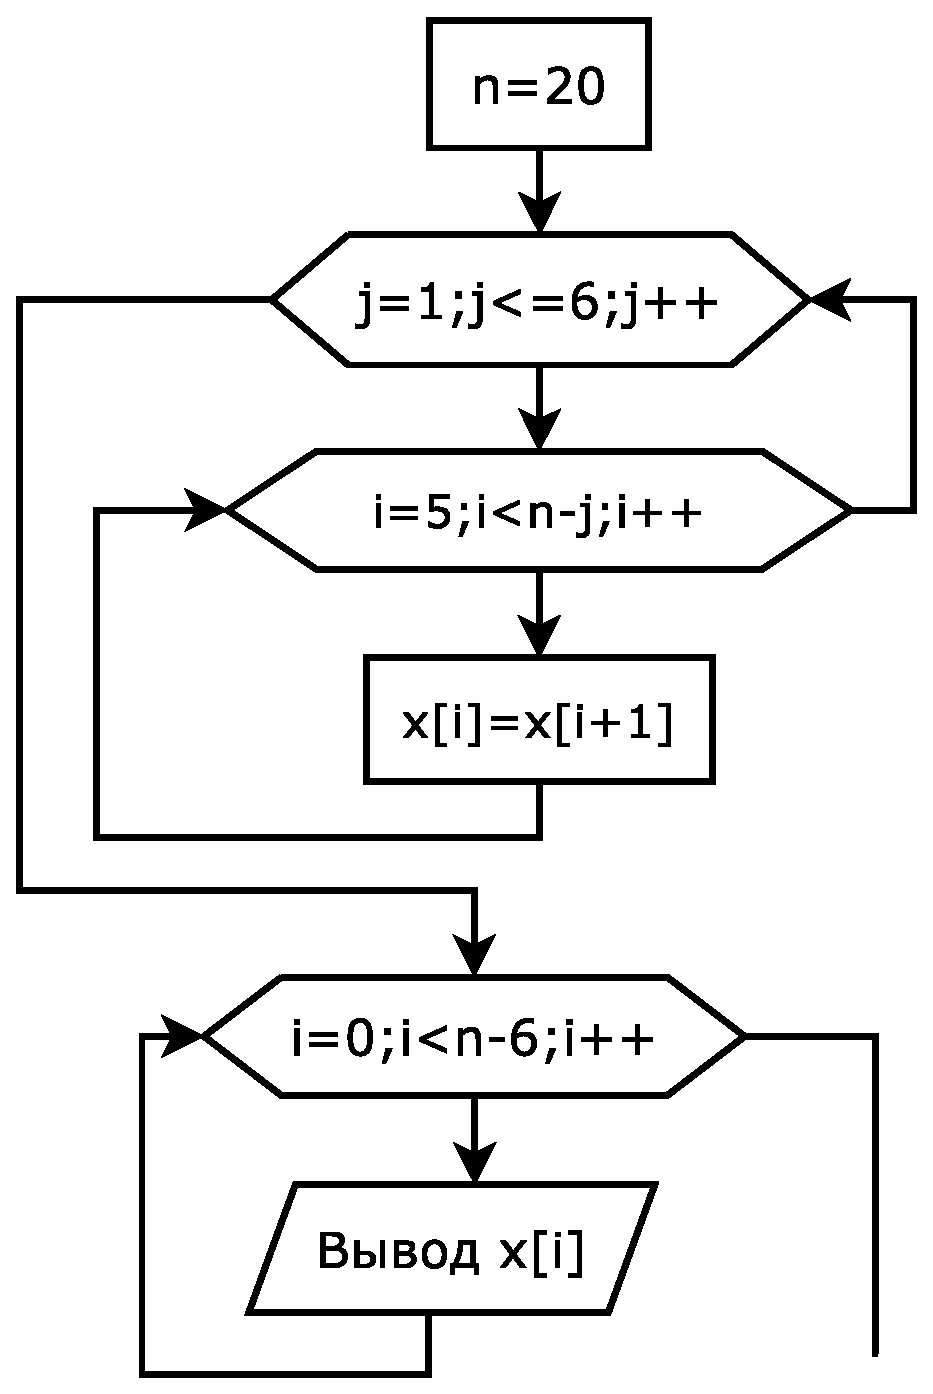
\includegraphics[width=0.5\textwidth]{img/ris_5_11}
\caption{Алгоритм решения задачи~\ref{gl05:prg5}}
\label{ch05:refDrawing10}
\end{center}
\end{figure}

\prg{Удалить из массива \Sys{X[n]} все положительные элементы.}{gl05:prg6}

При удалении отдельных элементов из массива следует учитывать: при удалении элемента (сдвиге элементов влево и
уменьшении $n$) не надо переходить к следующему, а если элемент не удалялся, то, наоборот, надо переходить к следующему.

Далее приведён текст программы решения задачи \ref{gl05:prg6}.
\begin{lstlisting}
#include <iostream>
#include <math.h>
using namespace std;
int main(int argc, char **argv)
{
  int i,j,n;
  cout<<"n=";cin>>n;
  float x[n];//`Выделяем память для динамического массива x.`
  cout<<"`\Sys{Введите элементы массива X}` \n"; //`Ввод элементов массива.`
  for(i=0;i<n;i++)
    cin>>x[i];
  for(i=0;i<n;)
    if (x[i]>0) //`Если текущий элемент положителен,`
    { //`то удаляем элемент с индексом i.`
      for(j=i;j<n-1;j++)
        x[j]=x[j+1];
      n--;
    }
    else i++; //`иначе --- переходим к следующему элементу массива.`	
  cout<<"`\Sys{Преобразованный массив X}` \n"; //`Вывод элементов массива.`
  for(i=0;i<n;i++)
    cout<<x[i]<<"\t";
  cout<<endl;
  return 0;
}
\end{lstlisting}


\prg{Удалить из массива все отрицательные элементы, расположенные между максимальным
и минимальным элементами массива \Sys{X[n]}.}{gl05:prg7}

Решение этой задачи можно разделить на следующие этапы:

\begin{enumerate}
\item Ввод массива.
\item Поиск номеров максимального (\Sys{nmax}) и минимального (\Sys{nmin}) элементов массива.
\item Определение меньшего (\Sys{a}) и большего (\Sys{b}) из чисел \Sys{nmax} и
\Sys{nmin}.
\item Далее, необходимо перебрать все элементы массива, расположенные между числами с номерами \Sys{a} и
\Sys{b}. Если число окажется отрицательным, то его необходимо удалить. Однако на этом этапе нужно
учитывать тонкий момент. Если просто организовать цикл от \Sys{a+1} до \Sys{b-1}, то при
удалении элемента изменяется количество элементов, расположенных между
\Sys{a} и \Sys{b}, и номер последнего удаляемого элемента. 
Это может привести к тому, что не всегда корректно будут удаляться
отрицательные элементы, расположенные между \Sys{a} и \Sys{b}. Поэтому этот цикл для удаления
организован несколько иначе.
\end{enumerate}

Текст программы:
\begin{lstlisting}
#include <iostream>
#include <math.h>
using namespace std;
int main(int argc, char **argv)
{
  int i,j,k,n,nmax,nmin, *x,a,b;
  cout<<"n="; cin>>n; //`Ввод количества элементов в массиве.`
  x=new int [n]; //`Выделяем память для динамического массива x.`
  cout<<"`\Sys{Введите элементы массива X}` \n"; //`Ввод элементов массива.`
  for(i=0;i<n;i++)
    cin>>x[i];
  //`Поиск номеров максимального и минимального элементов в массиве.`
  for(nmax=nmin=i=0;i<n;i++)
  {
    if (x[i]<x[nmin]) nmin=i;
    if (x[i]>x[nmax]) nmax=i;
  }
  //`Проверяем, что раньше расположено, минимум или максимум`
  if (nmin<nmax) 
  {
    a=nmin;
    b=nmax;
  }
  else
  {
    a=nmax;
    b=nmin;
  } 
  //`Перебираем все элементы, расположенные между максимумом и минимумом`
  for(i=a+1,k=1;k<=b-a-1;k++)
    if (x[i]<0) //`Проверяем, является ли очередной элемент массива отрицательным.`
    {//`Если текущий элемент массива является отрицательным числом, удаляем его`
      for(j=i;j<n-1;j++)
        x[j]=x[j+1];
      n--;
    }
    else i++; //`Если x[i]>=0, переходим к следующему элементу.`
  cout<<"`\Sys{Преобразованный массив X}`\n";
  for(i=0;i<n;i++)
    cout<<x[i]<<"\t";
  cout<<endl;	
  return 0;
}
\end{lstlisting}

В качестве тестового можно использовать следующий массив: 
$34, 4, -7, -8, -10, 7, -100, -200, -300, 1$. Здесь приведённая
выше программа работает корректно, а вариант 
\begin{lstlisting}
for(i=a+1;i<b;) 
  if (x[i]<0) 
  { 
    for(j=i;j<n-1;j++)
      x[j]=x[j+1]; 
    n--;
  }
  else i++;
\end{lstlisting}
приводит к неправильным результатам. Рекомендуем читателю самостоятельно разобраться в особенностях подобных алгоритмов
удаления.

\prg{В массиве \Sys{X[n]} найти группу наибольшей длины, которая состоит из
знакочередующихся чисел.}{gl05:prg8}

Если будут вычислены следующие значения:
\begin{itemize}
\item \Sys{nach} --- номер первого элемента в группе;
\item \Sys{kon} --- номер последнего элемента в группе;
\item \Sys{k} --- количество элементов в группе.
\end{itemize}
то, зная любые два из них, можно однозначно определить группу внутри массива.

Вначале количество элементов в знакочередующейся группе равно 1. Дело в том, что если мы встретим первую пару
знакочередующихся элементов, то количество их в группе сразу станет равным 2. Однако все последующие пары элементов
будут увеличивать \Sys{k} на 1. И чтобы не решать проблему построения последовательности значений
\Sys{k} 0,2,3,4,5,..., первоначальное значение \Sys{k} примем равным 1. Когда будем встречать
очередную пару подряд идущих соседних элементов, то \Sys{k} необходимо будет увеличить на 1.

Алгоритм поиска очередной группы состоит в следующем: попарно ($x_i$, $x_{i+1})$ перебираем все элементы массива
(параметр цикла $i$ изменяется от 0 до $n-2$). 

Если произведение соседних элементов отрицательно ($x_i\cdot x_{i+1} < 0$), то это означает, что они имеют разные знаки и
являются элементами группы. В этом случае количество $(k)$ элементов в группе увеличиваем на 1 (\Sys{k++}).
Если же произведение соседних элементов положительно ($x_i\cdot x_{i+1} > 0$), то эти элементы не являются членами
группы. В этом случае возможны два варианта:

\begin{enumerate}
\item Если  $k>1$, то только что закончилась группа, в этом случае \Sys{kon=i} --- номер последнего элемента
в группе, $k$ --- количество элементов в только что закончившейся группе.
\item Если  $k=1$, то это просто очередная пара незнакочередующихся элементов.
\end{enumerate}
После того, как закончилась очередная группа знакочередующихся элементов, необходимо количество групп
(\Sys{kgr}) увеличить на 1 (\Sys{kgr++}). Если это первая группа (\Sys{kgr=1})
знакочередующихся элементов, то в переменную \Sys{max} записываем длину этой группы
(\Sys{max=k})\footnote{В переменной}, а в переменную
\Sys{kon\_max} номер последнего элемента группы
(\Sys{kon\_max=i}). Если это не первая группа
(\Sys{kgr=1}), то сравниваем \Sys{max} и длину текущей группы
(\Sys{k}). Если \Sys{k>max}, то в переменную \Sys{max}
записываем длину этой группы (\Sys{max=k}), а в переменную
\Sys{kon\_max} номер последнего элемента группы
(\Sys{kon\_max=i}). 

После этого в переменную \Sys{k} опять записываем 1 для формирования новой группы
элементов.

По окончанию цикла значение \Sys{k} может быть больше 1. Это означает, что в самом конце массива
встретилась ещё одна группа. Для неё надо будет провести все те же действия, что и для любой другой группы. Далее
приведён текст программы.
\begin{lstlisting}
#include <iostream>
using namespace std;
int main(int argc, char **argv)
{ float *x;
  int i,k,n,max,kgr,kon_max;
  cout<<"n=";cin>>n; //`Ввод размера массива.`
  x=new float [n];  //`Выделение памяти для массива.`
  cout<<"`Введите массив x`\n";  //`Ввод элементов массива.`
  for(i=0;i<n;i++)
    cin>>x[i];
  //`Попарно перебираем элементы массива. Количество знакочередующихся` 
  //`групп в массиве kgr=0, количество элементов в текущей группе --- 1.`
  for(kgr=i=0,k=1;i<n-1;i++)
    //`Если соседние элементы имеют разные знаки, то количество (k)` 
    //`элементов в группе увеличиваем на 1.`
    if (x[i]*x[i+1]<0) k++;
    else
      if (k>1) //`Если k>1, то только что закончилась группа, i --- номер последнего элемента` 
      {//`в группе, k --- количество элементов в группе. Увеличиваем kgr на 1.`
        kgr++;
        if (kgr==1) //`Если это первая группа (kgr=1) знакочередующихся элементов,`
        {
          max=k; //`то max --- длина группы (max=k),`
          kon_max=i; //`kon\_max --- номер последнего элемента группы.`
        }
        else //`это не первая группа ($kgr\ne 1$), сравниваем max и длину текущей группы.`
          if (k>max) //`Если k>max,`
          {
            max=k; //`max --- длина группы,`
            kon_max=i; //`kon\_max --- номер последнего элемента группы.`
          }
        k=1; //`В переменную k записываем 1 для формирования новой группы элементов.`
      }
    if (k>1) //`Если в конце массива была группа.` 
    {
      kgr++; //`Количество групп увеличиваем на 1.`
      if (kgr==1) //`Если это первая группа,`
      {
        max=k; //`то max --- длина группы,`
        kon_max=n-1; //`группа закончилась на последнем элементе массива.`
      }
      else
        if (k>max) //`Если длина очередной группы больше max.`
        {
          max=k; //`то в max записываем длину последней группы,`
          kon_max=n-1; //`группа закончилась на последнем элементе массива.`
        }
    }
    if (kgr>0) //`Если знакочередующиеся группы были,`
    { //`то выводим информацию о группе наибольшей длины,`
      cout<<"`В массиве `"<<kgr<<"` групп знакочередующихся элементов`\n";
      cout<<"`Группа максимальной длины начинается с элемента Номер `"<<kon_max-max+1<<",` её длина `"<<max<<"` ,номер последнего элемента группы `" <<kon_max<<endl;
      for(i=kon_max-max+1;i<=kon_max;i++) //`а также саму группу.`
        cout<<x[i]<<" ";
      cout<<endl;		
    }
    else //`Если знакочередующихся групп не было, то выводим сообщение об этом.` 
      cout<<"`\Sys{В массиве нет групп знакочередующихся элементов}`\n";
  return 0;
}
\end{lstlisting}

\subsection[Сортировка элементов в массиве]{Сортировка элементов в массиве}
\index{Алгоритм!Сортировка элементов массива}Сортировка представляет собой процесс упорядочения элементов в массиве в
порядке возрастания или убывания их значений. Например, массив $Y$ из $n$ элементов
будет отсортирован в порядке возрастания значений его элементов, если

 $Y[0]<Y[1]<{\dots}<Y[n-1]$,

и в порядке убывания, если

 $Y[0]>Y[1]>{\dots}>Y[n-1]$.

Существует большое количество алгоритмов сортировки, но все они базируются на трёх основных:

\begin{itemize}
\item сортировка обменом;
\item сортировка выбором;
\item сортировка вставкой.
\end{itemize}

Представим, что нам необходимо разложить по порядку карты в колоде. Для сортировки карт \emph{обменом} можно разложить
карты на столе лицевой стороной вверх и менять местами те карты, которые расположены в неправильном порядке, делая это
до тех пор, пока колода карт не станет упорядоченной.

Для \emph{сортировки выбором} из разложенных на столе карт выбирают самую младшую (старшую) карту и держат её в руках.
Затем из оставшихся карт вновь выбирают наименьшую (наибольшую) по значению карту и помещают её позади той карты,
которая была выбрана первой. Этот процесс повторяется до тех пор, пока вся колода не окажется в руках. Поскольку каждый
раз выбирается наименьшая (наибольшая) по значению карта из оставшихся на столе карт, по завершению такого процесса
карты будут отсортированы по возрастанию (убыванию).

Для \emph{сортировки вставкой} из колоды берут две карты и располагают их в необходимом порядке по отношению друг к
другу. Каждая следующая карта, взятая из колоды, должна быть установлена на соответствующее место по отношению к уже
упорядоченным картам.

Итак, решим следующую задачу. Задан массив $Y$ из $n$ целых чисел. Расположить элементы массива в порядке возрастания их
значений.

\subsubsection[Сортировка методом «пузырька»]{Сортировка методом «пузырька»}
Сортировка пузырьковым методом является наиболее известной. Её популярность объясняется запоминающимся названием,
которое происходит из-за подобия процессу движения пузырьков в резервуаре с водой, когда каждый пузырёк находит свой
собственный уровень, и простотой алгоритма. Сортировка методом «пузырька» использует метод обменной сортировки и
основана на выполнении в цикле операций сравнения и при необходимости обмена соседних элементов. Рассмотрим алгоритм
пузырьковой сортировки более подробно.

Сравним нулевой элемент массива с первым, если нулевой окажется больше первого, то поменяем их местами. Те же действия
выполним для первого и второго, второго и третьего, $i$–го и ($i+1)$–го,
предпоследнего и последнего элементов. В результате этих действий самый большой элемент станет на последнее
($n-1)$-е место. Теперь повторим данный алгоритм сначала, но последний ($n-1)$-й
элемент рассматривать не будем, так как он уже занял своё место. После проведения данной операции самый большой
элемент оставшегося массива станет на ($n-2)$-е место. Так повторяем до тех пор, пока не упорядочим
весь массив.

В табл.~\ref{ch05:refTable3} представлен процесс упорядочивания элементов в массиве. 

{\noindent\small
\begin{longtable}{|p{0.3\textwidth}|c|c|c|c|c|}
\caption{Процесс упорядочивания элементов} \label{ch05:refTable3}\\
\hline
\endfirsthead
\multicolumn{6}{c}%
{{\tablename\ \thetable{} --- продолжение}} \\
\hline
\endhead
\Emph{Номер элемента} &\Emph{0} &\Emph{1} &\Emph{2} &\Emph{3} &\Emph{4}\\\hline
Исходный массив &7 &3 &5 &4 &2\\\hline
Первый просмотр &3 &5 &4 &2 &7\\\hline
Второй просмотр &3 &4 &2 &5 &7\\\hline
Третий просмотр &3 &2 &4 &5 &7\\\hline
Четвёртый просмотр &2 &3 &4 &5 &7\\\hline
\end{longtable}
}

Нетрудно заметить, что для преобразования массива, состоящего из $n$ элементов, необходимо просмотреть его
$n-1$ раз, каждый раз уменьшая диапазон просмотра на один элемент. Блок–схема описанного алгоритма
приведена на рис.~\ref{ch05:refDrawing11}. 

\begin{figure}[htb]
\begin{center}
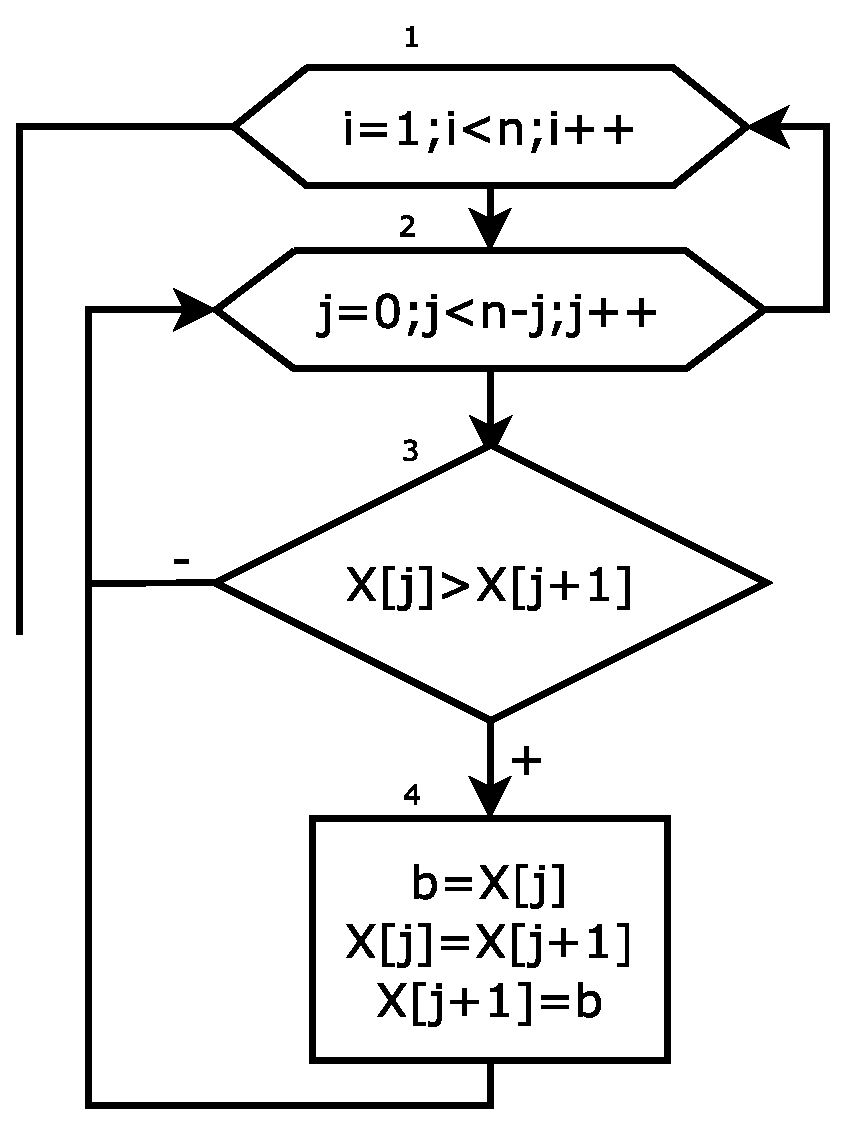
\includegraphics[width=0.3\textwidth]{img/ris_5_12}
\caption{Сортировка массива пузырьковым методом}
\label{ch05:refDrawing11}
\end{center}
\end{figure}

Обратите внимание на то, что для перестановки элементов (рис.~\ref{ch05:refDrawing11}, блок 4) используется буферная
переменная $b$, в которой временно хранится значение элемента, подлежащего замене. Текст программы, сортирующей элементы
в массиве по возрастанию методом «пузырька», приведён далее.
\begin{lstlisting}
#include <iostream>
using namespace std;
int main()
{
  int n,i,b,j;
  cout<<" n="; cin>>n;
  float y[n];
  for (i=0;i<n;i++)   //`Ввод массива.`
  {
    cout<<"\n Y["<<i<<"]=";
    cin>>y[i];
  }
  for(j=1;j<n;j++) //`Упорядочивание элементов в массиве по возрастанию их значений.`
    for(i=0;i<n-j;i++)
      if (y[i]>y[i+1]) //`Если текущий элемент больше следующего`
      {
        b=y[i]; //`Сохранить значение текущего элемента`
        y[i]=y[i+1]; //`Заменить текущий элемент следующим`
        y[i+1]=b; //`Заменить следующий элемент на сохранённый в \Sys{b}`
      }
  for (i=0;i<n;i++) cout<<y[i]<<"\t"; //`Вывод упорядоченного массива`
  return 0;
}
\end{lstlisting}

Для перестановки элементов в массиве по убыванию их значений необходимо в программе и блок-схеме при сравнении элементов
массива заменить знак <<{>}>> на <<{<}>>.

Однако, в этом и во всех далее рассмотренных алгоритмах не учитывается то факт, что на каком-то этапе (или даже в начале)
массив уже может оказаться отсортированным. При большом количестве элементов (сотни и даже тысячи чисел) на
\emph{сортировку «вхолостую»} массива тратится достаточно много времени. Ниже приведены тексты двух
вариантов программы сортировки по убыванию методом пузырька, в которых алгоритм прерывается, если массив уже
отсортирован.

Вариант 1.
\begin{lstlisting}
#include <iostream>
using namespace std;
int main(int argc, char **argv)
{
  int n,i,b,j;
  bool pr;
  cout<<" n="; cin>>n;
  float y[n];
  for (i=0;i<n;i++)  //`Ввод массива.`
  {
    cout<<"\n Y["<<i<<"]=";
    cin>>y[i];
  }
  for(j=1;j<n;j++) //`Упорядочивание элементов массива по убыванию их значений.`
  {
    for(pr=false, i=0;i<n-j;i++) //`Предполагаем, что массив уже отсортирован`
                                 //(pr=false).
      if (y[i]<y[i+1])//`Если текущий элемент меньше следующего`
      {
        b=y[i]; //`Сохранить значение текущего элемента`
        y[i]=y[i+1]; //`Заменить текущий элемент следующим`
        y[i+1]=b; //`Заменить следующий элемент текущим`
        pr=true; //`Если элемент менялись местами, массив ещё не отсортирован (\Sys{pr=true});`
      }
    cout<<"j="<<j<<endl;
    //`Если на j-м шаге соседние элементы не менялись, то массив уже отсортирован,`
    if (!pr) break; //`повторять смысла нет;`
  }
  for (i=0;i<n;i++) cout<<y[i]<<"\t"; //`Вывод упорядоченного массива`
  return 0;
}
\end{lstlisting}

Вариант 2.
\begin{lstlisting}
#include <iostream>
using namespace std;
int main(int argc, char **argv)
{
  int n,i,b,j;
  bool pr=true;
  cout<<" n="; cin>>n;
  float y[n];
  for (i=0;i<n;i++) //`Ввод массива.`
  {
    cout<<"\n Y["<<i<<"]=";
    cin>>y[i];
  }
  for(j=1;pr;j++) //`Упорядочивание элементов массива по убыванию их значений.`
  { //`Вход в цикл, если массив не отсортирован (pr=true).`
    for(pr=false, i=0;i<n-j;i++) //`Предполагаем, что массив уже отсортирован`  
                                 //(pr=false).
      if (y[i]<y[i+1])//`Если текущий элемент меньше следующего`
      {
        b=y[i]; //`Сохранить значение текущего элемента`
        y[i]=y[i+1]; //`Заменить текущий элемент следующим`
        y[i+1]=b; //`Заменить следующий элемент текущим`
        pr=true; //`Элементы менялись местами, массив ещё не отсортирован` (pr=true)
      }
  }
  for (i=0;i<n;i++) cout<<y[i]<<"\t";//`Вывод упорядоченного массива`
  return 0;
}
\end{lstlisting}

\subsubsection[Сортировка выбором]{Сортировка выбором}
Алгоритм сортировки выбором приведён в виде блок-схемы на рис.~\ref{ch05:refDrawing12}. Идея алгоритма заключается в
следующем. В массиве $Y$, состоящем из $n$ элементов, ищем самый большой элемент (блоки
2--5) и меняем его местами с последним элементом (блок 7). Повторяем алгоритм поиска максимального элемента, но
последний ($n-1)$-й элемент не рассматриваем, так как он уже занял свою позицию. 

\begin{figure}[htb]
\begin{center}
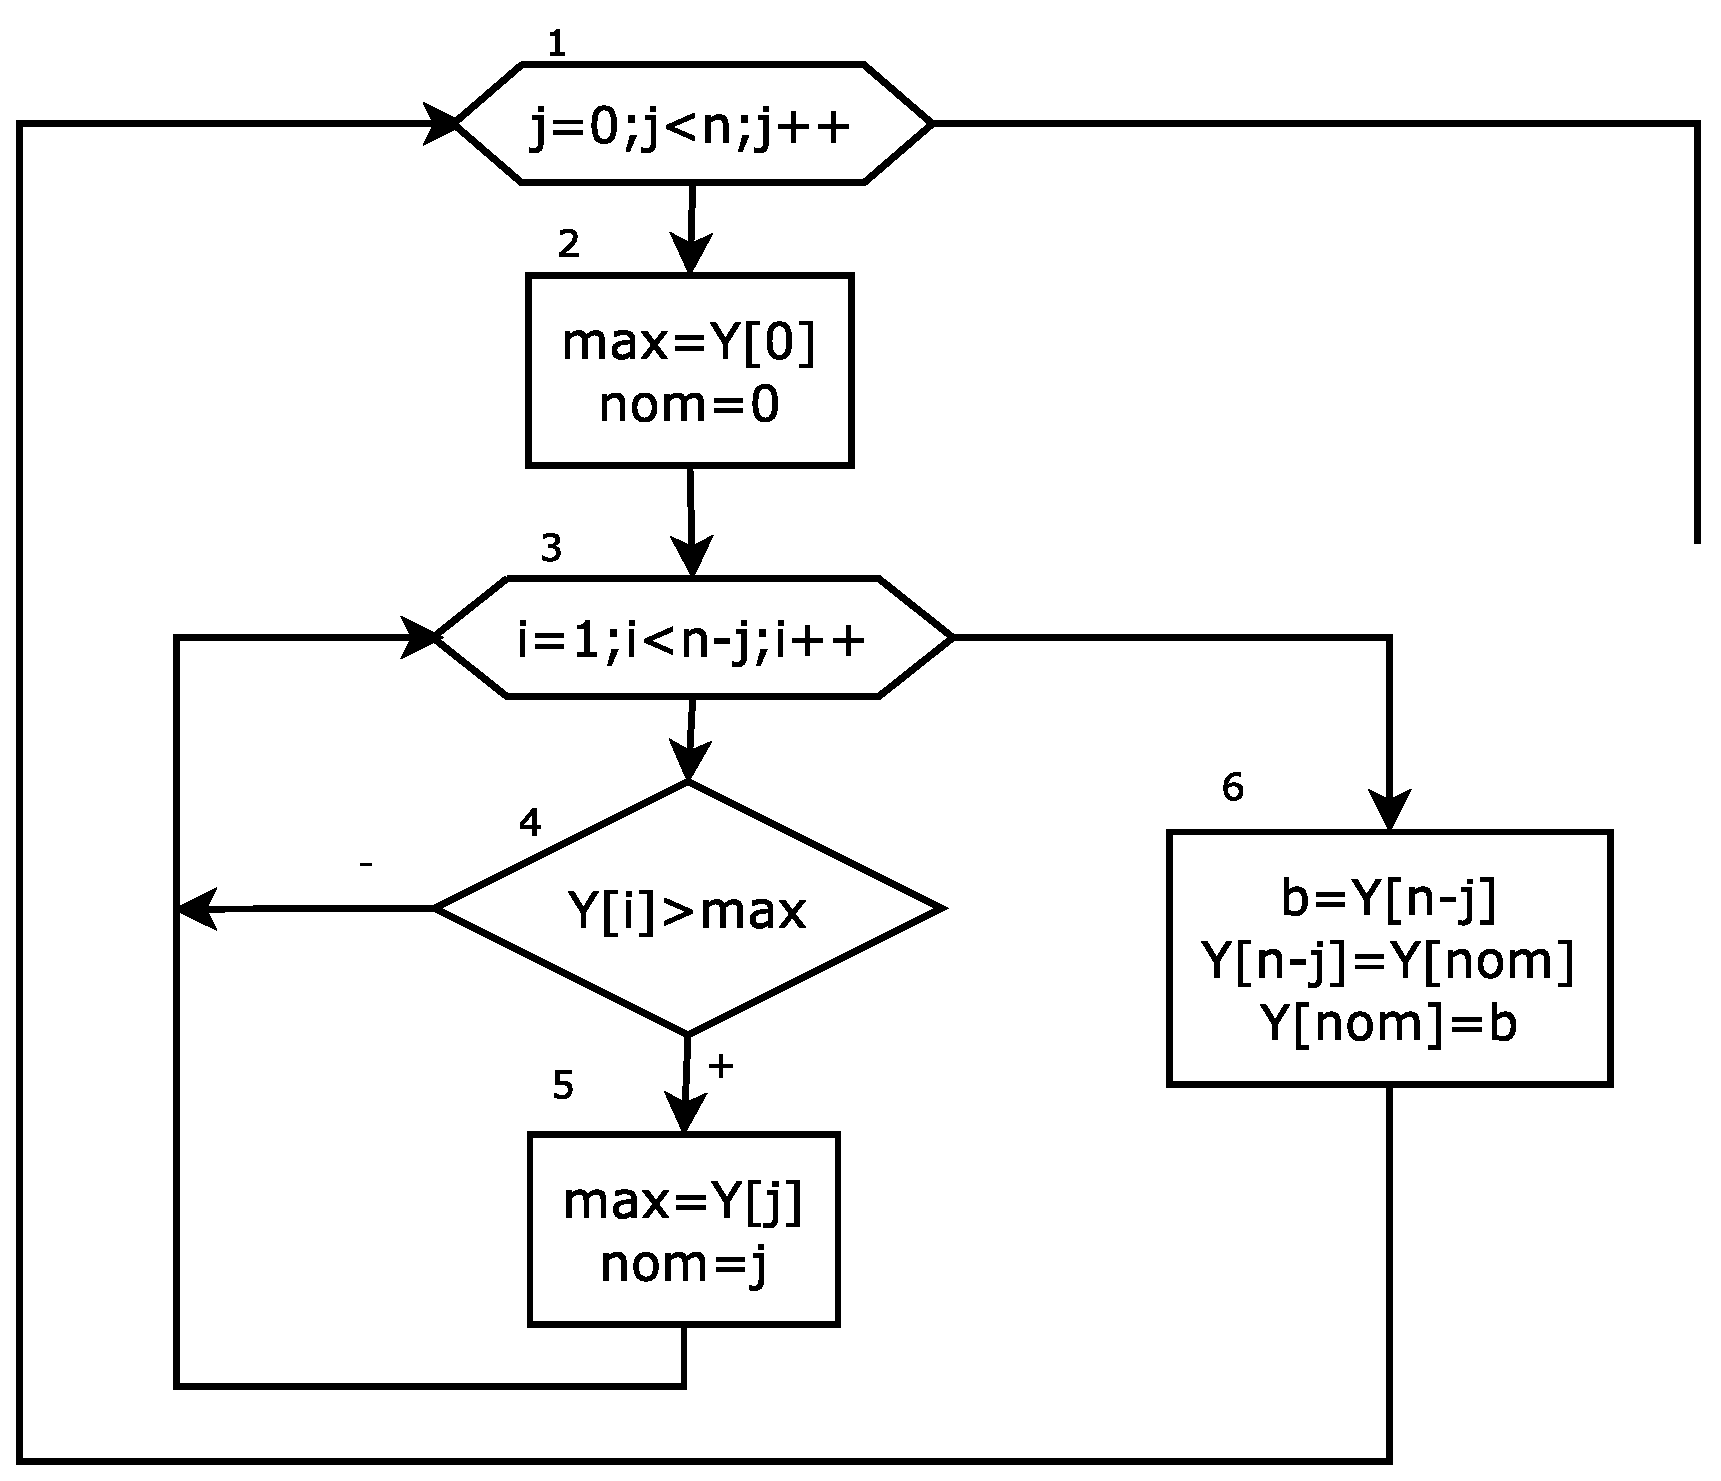
\includegraphics[width=0.5\textwidth]{img/ris_5_13}
\caption{Сортировка массива выбором наибольшего элемента}
\label{ch05:refDrawing12}
\end{center}
\end{figure}

Найденный максимум ставим на ($n-2)$-ю позицию. Описанную выше операцию поиска проводим
$n-1$ раз, до полного упорядочивания элементов в массиве. Фрагмент программы выполняет сортировку
массива по возрастанию методом выбора:
\begin{lstlisting}
for(j=1;j<n;b=y[n-j],y[n-j]=y[nom],y[nom]=b,j++)
  for(max=y[0],nom=0,i=1;i<=n-j;i++) 
    if (y[i]>max) {max=y[i];nom=i;}
\end{lstlisting}

Для упорядочивания массива по убыванию необходимо менять минимальный элемент с последним элементом.

\subsubsection[Сортировка вставкой]{Сортировка вставкой}
Сортировка вставкой заключается в том, что сначала упорядочиваются два элемента массива. Затем делается вставка третьего
элемента в соответствующее место по отношению к первым двум элементам. Четвёртый элемент помещают в список из уже
упорядоченных трёх элементов. Этот процесс повторяется до тех пор, пока все элементы не будут упорядочены. 

Прежде чем приступить к составлению блок–схемы, рассмотрим следующий пример. Пусть известно, что в массиве из десяти
элементов первые шесть уже упорядочены (с нулевого по пятый), а шестой элемент нужно вставить между вторым и четвёртым.
Сохраним шестой элемент во вспомогательной переменной, а на его место запишем пятый. Далее четвёртый переместим на
место пятого, а третий на место четвёртого, тем самым выполнив сдвиг элементов массива на одну позицию вправо. Записав
содержимое вспомогательной переменной в третью позицию, достигнем нужного результата.

Составим блок–схему алгоритма (рис.~\ref{ch05:refDrawing13}), учитывая, что возможно описанные выше действия придётся
выполнить неоднократно.

\begin{figure}[htb]
\begin{center}
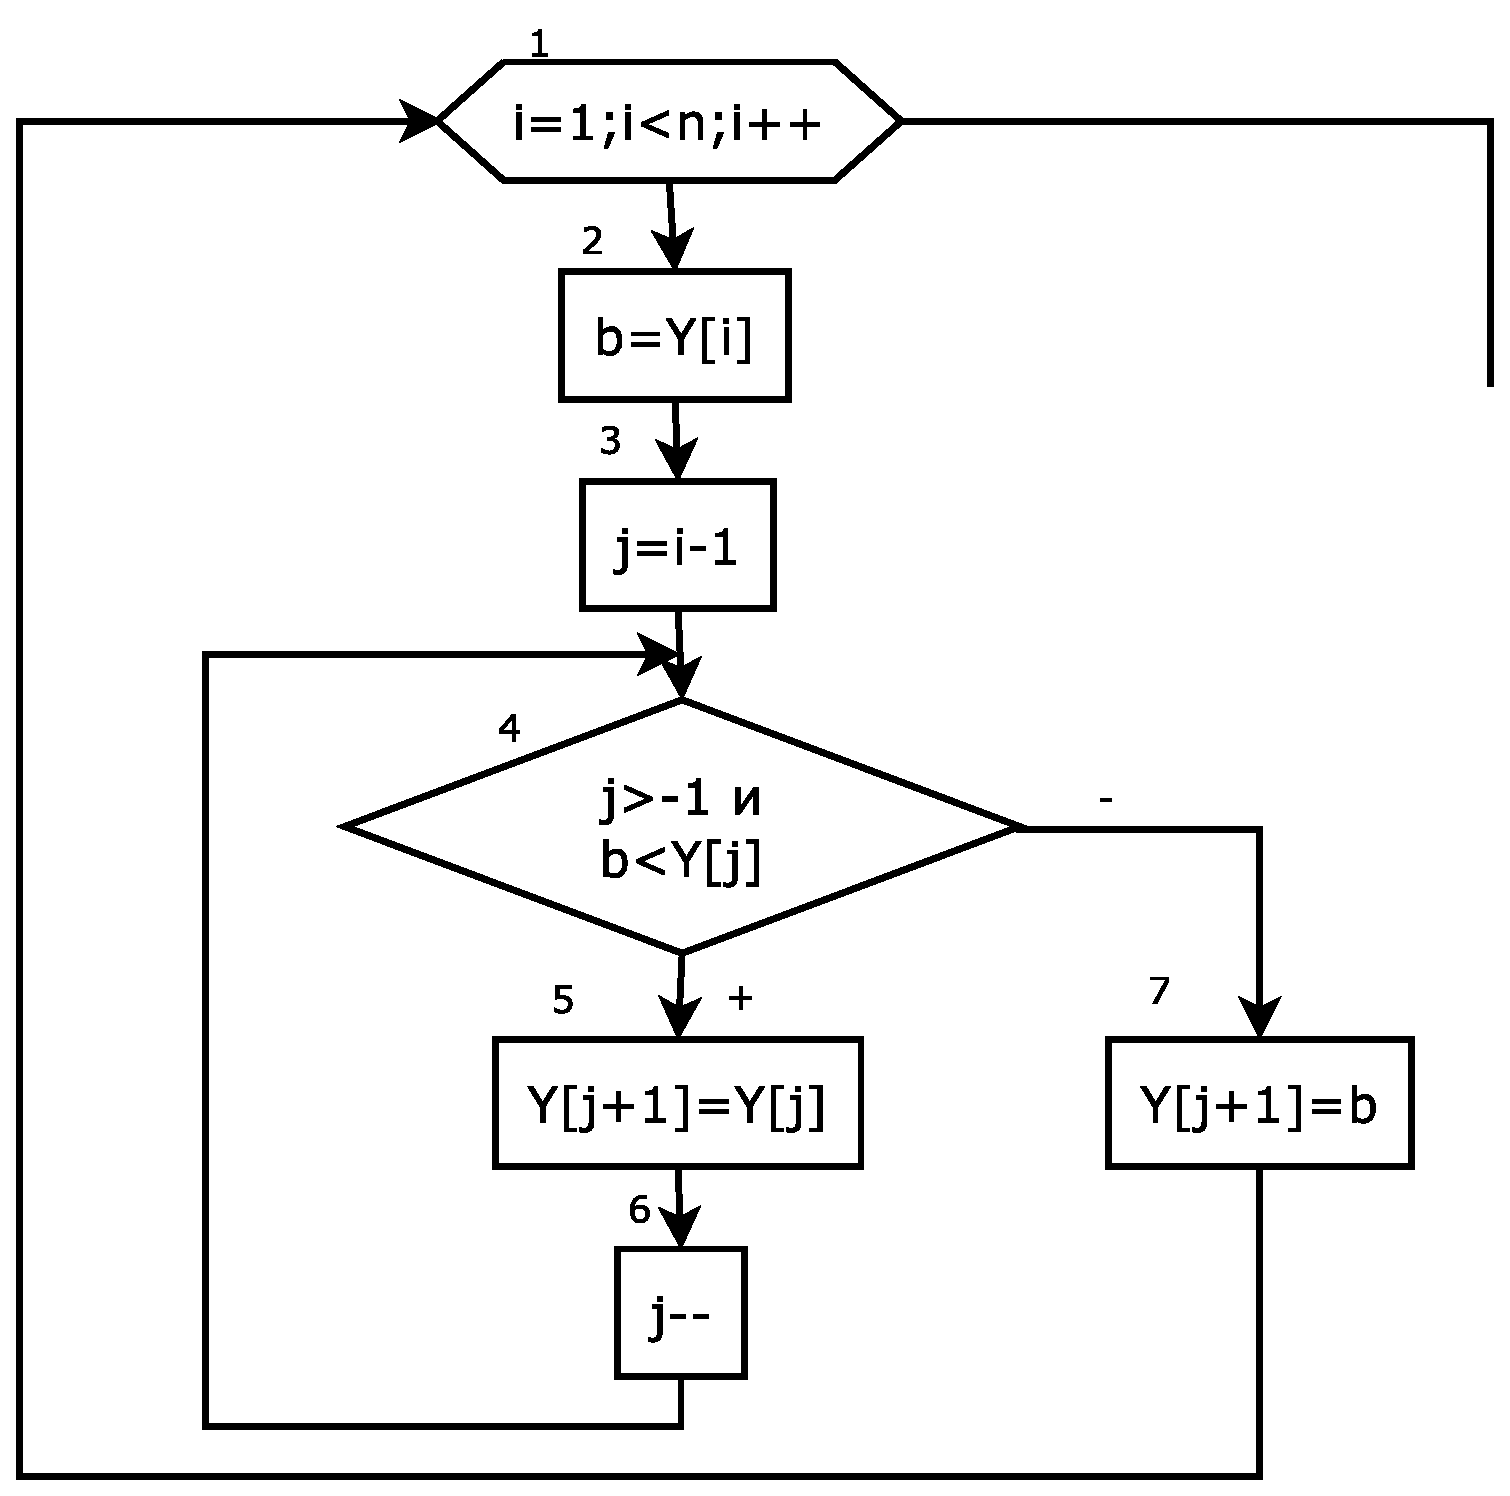
\includegraphics[width=0.5\textwidth]{img/ris_5_14}
\caption{Сортировка массива вставкой}
\label{ch05:refDrawing13}
\end{center}
\end{figure}


 Организуем цикл для просмотра всех элементов массива, начиная с первого (блок~1). Сохраним значение текущего
$i$–го элемента во вспомогательной переменной $b$, так как оно может быть потеряно
при сдвиге элементов (блок 2), и присвоим переменной $j$ значение индекса предыдущего
($i-1)$–го элемента массива (блок 3). Далее движемся по массиву влево в поисках элемента, меньшего чем
текущий, и, пока он не найден, сдвигаем элементы вправо на одну позицию. Для этого организуем цикл (блок~4), который
прекратиться, как только будет найден элемент меньше текущего. Если такого элемента в массиве не найдётся и переменная
$j$ станет равной ($-1$), то это будет означать, что достигнута левая граница массива, и текущий элемент
необходимо установить в первую позицию. Смещение элементов массива вправо на одну позицию выполняется в блоке~5, а
изменение счётчика $j$ в блоке~6. Блок~7 выполняет вставку текущего элемента в соответствующую
позицию.
Далее приведён фрагмент программы, реализующей сортировку массива методом вставки.
\begin{lstlisting}
for(i=1;i<n;y[j+1]=b,i++) 
  for(b=y[i],j=i-1;(j>-1 && b<y[j]);y[j+1]=y[j],j--);
\end{lstlisting}

Рассмотрим несколько несложных задач, связанных с упорядочиванием.

\prg{Задан массив $a[n]$, упорядоченный по убыванию, вставить в него некоторое
число $b$, не нарушив упорядоченности массива.}{gl05:prg9}

Массив является упорядоченным по убыванию, если каждое последующий элемент массива не больше предыдущего, т.~е. при
выполнении следующей совокупности неравенств $a_0\geqslant a_1\geqslant a_2\geqslant ...\geqslant a_{n-3}\geqslant a_{n-2}\geqslant a_{n-1}$. 

Для вставки в подобный массив некоторого числа без нарушений упорядоченности, необходимо:

\begin{enumerate}
\item Найти номер $k$ первого числа в массиве, которое  $a_{k}\leqslant b$.
\item Все элементы массива $a$, начиная от $n-1$ до $k$-го, сдвинуть
на один вправо\footnote{Очень важно, что сдвиг осуществляем от $n-1$-го до $k$-го, в противном случае элементы массива
оказались бы испорченными.}.
\item На освободившееся место с номером $k$ записать число $b$.
\end{enumerate}
Текст программы с комментариями приведён ниже.
\begin{lstlisting}[numbers=left, numberstyle=\tiny, stepnumber=2, numbersep=5pt] 
#include <iostream>
using namespace std;
int main(int argc, char **argv)
{
  int i,k,n;
  float b;
  cout<<"n=";cin>>n; //`Ввод размера исходного массива.`
  float a[n+1]; //`Выделение памяти с учётом предстоящей вставки одного числа в массив.`
  cout<<"`\Sys{Введите массив }`a\n"; //`Ввод исходного упорядоченного по убыванию массива.`
  for(i=0;i<n;i++)
    cin>>a[i];
  cout<<"`\Sys{Введите число}` b=";cin>>b; //`Ввод вставляемого в массив числа b`.
  //`Если число b меньше всех элементов массива, записываем b в последний элемент массива.`
  if (a[n-1]>=b) a[n]=b;
  else //`Иначе`
  {
    for(i=0;i<n;i++) //`Ищем первое число, меньшее` b.
      if (a[i]<=b) 
      {
        k=i; //`Запоминаем его номер в переменной` k.
        break;
      }
    for(i=n-1;i>=k;i--) //`Все элементы массива от $n-1$-го до $k$-го сдвигаем на один вправо.`
      a[i+1]=a[i];
    a[k]=b; //`Вставляем число $b$ в массив.`
  }
  cout<<"`\Sys{Преобразованный массив}` a\n";
  for(i=0;i<=n;i++)
    cout<<a[i]<<"\t";
  return 0;
}
\end{lstlisting}

Обратите внимание, при решении задачи с массивом, упорядоченным по возрастанию необходимо во 
фрагменте со строки 14 по строку 22
заменить все операции отношения на противоположные.

\prg{Проверить, является ли массив упорядоченным по возрастанию.}{gl05:prg10}

Для проверки упорядоченности по возрастанию \Sys{a[n]}\footnote{Массив является упорядоченным по
возрастанию, если выполняются условия  $a_0\leqslant a_1\leqslant a_2\leqslant ...\leqslant a_{n-3}\leqslant a_{n-2}\leqslant a_{n-1}$.} можно
поступить следующим образом. Предположим, что массив упорядочен (\Sys{pr=true}). Если хотя бы для одной
пары соседних элементов выполняется условие $a_i>a_{i+1}$, то массив не упорядочен по возрастанию
(\Sys{pr=false}). Текст программы с комментариями приведён ниже. Читателю предлагается преобразовать
программу таким образом, чтобы осуществлялась проверка, упорядочен ли массив по убыванию.
\begin{lstlisting}
#include <iostream>
using namespace std;
int main(int argc, char **argv)
{
  int i,n;
  bool pr;
  cout<<"n=";cin>>n; //`Ввод размера исходного массива.`
  float *a=new float [n]; //`Выделение памяти для массива.`
  cout<<"`\Sys{Введите массив}` a\n"; //`Ввод исходного массива.`
  for(i=0;i<n;i++)
    cin>>a[i];
  //`Предполагаем, что массив упорядочен (\Sys{pr=true}), перебираем все пары соседних значений`
  //`(\Sys{i} --- номер пары), при \Sys{i} равном $n-2$ будем сравнивать последнюю пару \Sys{a[n-2]} и \Sys{a[n-1]}.`
  for(pr=true,i=0;i<n-1;i++)
  //`Если для очередной пары соседних элементов выяснилось, что предыдущий элемент больше` 
  //`последующего, то массив неупорядочен по возрастанию (pr=false), остальные пары соседних` 
  //`значений, можно не проверять (оператор break)` 
    if (a[i]>a[i+1]) {pr=false;break;}
  if (pr) cout<<"`\Sys{Массив упорядочен по возрастанию}`";
  else cout<<"`\Sys{Массив не упорядочен по возрастанию}`";
  return 0;
}
\end{lstlisting}

\section[Указатели на функции]{Указатели на функции}
При решении некоторых задач возникает необходимость передавать имя функции как параметр. В этом случае формальным
параметром является указатель на передаваемую функцию. В общем виде прототип указателя на функцию можно записать так.
\begin{lstlisting}
type (*name_f)(type1, type2, type3,...)
\end{lstlisting}
Здесь

\Sys{name\_f} --- имя функции

\Sys{type} --- тип, возвращаемый функцией, 

\Sys{type1, type2, type3,...} --- типы формальных параметров функции.

В качестве примера рассмотрим решение широко известной математической задачи.

\prg{Вычислить  $\int\limits_a^b f(x)dx$  методами Гаусса и Чебышёва.}{gl05:prg11}

Кратко напомним читателю методы численного интегрирования.

Метод Гаусса состоит в следующем. Определённый интеграл непрерывной функции на интервале от -1 до 1 можно заменить
суммой и вычислить по формуле  $\int\limits_{-1}^1 f(x)dx=\sum\limits_{i=1}^n A_if(t_i)$, $t_i$ --- точки из
интервала $[-1,1]$,  $A_i$ --- рассчитываемые коэффициенты. Методика определения  $A_i$,  $t_i$ представлена в~\cite{DM}.
Для практического использования значения коэффициентов при  $n=2,3,4,5,6,7,8$ представлены в табл.~\ref{ch05:refTable4}.

{\noindent\tabcolsep=0.3em\noindent\small
\begin{longtable}{|c|p{0.46\textwidth}|p{0.46\textwidth}|}
\caption{Значения коэффициентов в квадратурной формуле Гаусса} \label{ch05:refTable4}\\
\hline
\Emph{n} & \Emph{Массив t} & \Emph{Массив A}\\ 
\hline
\endfirsthead
\multicolumn{3}{c}%
{{\tablename\ \thetable{} --- продолжение}} \\
\hline
\Emph{n} & \Emph{Массив t} & \Emph{Массив A}\\ 
\hline
\endhead
\scriptsize{2} &\scriptsize{$-0.57735027$, $0.57735027$  }&\scriptsize{$1$, $1$}\\\hline
\scriptsize{3} &\scriptsize{$-0.77459667$, $0$, $0.77459667$} & \scriptsize{$5/9$, $8/9$, $5/9$}\\\hline
\scriptsize{4} &\scriptsize{$-0.86113631$, $-0.33998104$, $0.33998104$,  $0.86113631$} &\scriptsize{$0.34785484$, $0.65214516$, $0.65214516$, $0.34785484$}\\\hline
\scriptsize{5 }&\scriptsize{$-0.90617985$, $-0.53846931$, $0$, $0.53846931$,  $0.90617985$ }&\scriptsize{$0.23692688$, $0.47862868$, $0.568888889$, $0.47862868$, $0.23692688$}\\\hline
\scriptsize{6 }&\scriptsize{$-0.93246951$, $-0.66120939$, $-0.23861919$,  $0.23861919$, $0.66120939$, $0.93246951$ }&\scriptsize{$0.17132450$, $0.36076158$, $0.46791394$, $0.46791394$, $0.36076158$, $0.17132450$}\\\hline
\scriptsize{$7$ }&\scriptsize{$-0.94910791$, $-0.74153119$, $-0.40584515$, $0$, $0.40584515$, $0.74153119$, $0.94910791$ }&\scriptsize{$0.12948496$, $0.27970540$, $0.38183006$, $0.41795918$, $0.38183006$, $0.27970540$, $0.12948496$}\\\hline
\scriptsize{$8$ }&\scriptsize{$-0.96028986$, $-0.79666648$, $-0.52553242$, $-0.18343464$, $0.18343464$, $0.52553242$,  $0.79666648$, $0.96028986$ }&\scriptsize{$0.10122854$, $0.22238104$, $0.31370664$, $0.36268378$, $0.36268378$, $0.31370664$, $0.22238104$, $0.10122854$}\\\hline
\end{longtable}
}

Для вычисления интеграла непрерывной функции на интервале от $a$ до $b$ квадратурная формула Гаусса может быть записана
следующим образом  $\int\limits_a^bf(x)dx=\frac{b-a}{2}\sum\limits_{i=1}^nA_if\left(\frac{b+a}{2}\cdot
{\frac{b-a}{2}}t_i\right)$, значения коэффициентов  $A_i$ и $t_i$ приведены в табл.~\ref{ch05:refTable4}.

При использовании квадратурной формулы Чебышёва, определённый интеграл непрерывной функции на интервале от $-1$ до $1$
записывается в виде следующей формулы  $\int\limits_{-1}^1f(x)dx=\frac{2}{n}\sum\limits_{i=1}^nf(t_{i})$, $t_{i}$ 
 --- точки из интервала $[-1,1]$. Формула Чебышёва для вычисления интеграла на интервале от $a$ до $b$ может быть 
записана так 
$\int\limits_{a}^{b}f(x)dx=\frac{b-a}{n}\sum\limits_{i=1}^{n}f\left(\frac{b+a}{2}\cdot {\frac{b-a}{2}}t_{i}\right)$
Методика определения  $t_i$  представлена в~\cite{DM}. Рассмотренные формулы имеют смысл при  $n=2,3,4,5,6,7,9$ ,
коэффициенты  $t_{i}$ представлены в табл.~\ref{ch05:refTable5}.

{\noindent\tabcolsep=0.3em\noindent\small
\begin{longtable}{|c|p{0.92\textwidth}|}
\caption{Значения коэффициентов в квадратурной формуле Чебышёва} \label{ch05:refTable5}\\
\hline
\Emph{n} & \Emph{Массив t}\\
\hline
\endfirsthead
\multicolumn{2}{c}%
{{\tablename\ \thetable{} --- продолжение}} \\
\hline
\Emph{n} & \Emph{Массив t}\\
\hline
\endhead
\scriptsize{$2$ }&\scriptsize{$-0.577350$, $0.577350$}\\\hline
\scriptsize{$3$ }&\scriptsize{$-0.707107$, $0$, $-0.707107$}\\\hline
\scriptsize{$4$ }&\scriptsize{$-0.794654$, $-0.187592$, $0.187592$, $0.794654$}\\\hline
\scriptsize{$5$ }&\scriptsize{$-0.832498$, $-0.374541$, $0$, $0.374541$, $0.832498$}\\\hline
\scriptsize{$6$ }&\scriptsize{$-0.866247$, $-0.422519$, $-0.266635$, $0.266635$, $0.422519$, $0.866247$}\\\hline
\scriptsize{$7$ }&\scriptsize{$-0.883862$, $-0.529657$, $-0.323912$, $0$, $0.323912$, $0.529657$, $0.883862$}\\\hline
\scriptsize{$9$ }&\scriptsize{$-0.911589$, $-0.601019$, $-0.528762$, $-0.167906$, $0$, $0.167906$, $0.528762$, $0.601019$, $0.911589$}\\\hline
\end{longtable}
}

Осталось написать функции вычисления определённого интеграла $\int\limits_{a}^{b}f(x)dx$  методами Гаусса и
Чебышёва. Далее приведены тексты функций и функция main(). В качестве тестовых использовались интегралы  
$\int\limits_{0}^{2}\sin ^{4}xdx\approx 0.9701$,  $\int\limits_{5}^{13}\sqrt{2x-1}dx\approx 32.667$ .
\begin{lstlisting}
#include <iostream>
#include <math.h>
using namespace std;
//`Функция вычисления определённого интеграла методом Чебышёва.`
//`$(a,b)$ --- интервал интегрирования, \Sys{*fn} --- указатель на функцию типа \Sys{double f (double)}.`
double int_chebishev(double a, double b, 
double (*fn)(double))
{
  int i,n=9;
  double s,
  t[9]={-0.911589, -0.601019, -0.528762, -0.167906, 0, 0.167906, 0.528762, 0.601019,  0.911589};
  for(s=i=0;i<n;i++)
    s+=fn((b+a)/2+(b-a)/2*t[i]);
  s*=(b-a)/n;
  return s;
}
//`Функция вычисления определённого интеграла методом Гаусса.`
//`$(a,b)$ --- интервал интегрирования, \Sys{*fn} --- указатель на функцию типа \Sys{double f (double)}`
double int_gauss(double a, double b, double (*fn)(double))
{
  int i,n=8;
  double s,
  t[8]={-0.96028986, -0.79666648, -0.52553242, -0.18343464, 0.18343464, 0.52553242,  0.79666648, 0.96028986},
  A[8]={0.10122854, 0.22238104, 0.31370664, 0.36268378, 0.36268378, 0.31370664, 0.22238104, 0.10122854};
  for(s=i=0;i<n;i++)
    s+=A[i]*fn((b+a)/2+(b-a)/2*t[i]);
  s*=(b-a)/2;
  return s;
}
//`Функции \Sys{f1} и \Sys{f2} типа double \Sys{f(double)}, указатели на которые будут передаваться`
//`в \Sys{int\_gauss} и \Sys{int\_chebishev}.`
double f1(double y)
{
  return sin(y)*sin(y)*sin(y)*sin(y);
}
double f2(double y)
{ 
  return pow(2*y-1,0.5); 
}

int main(int argc, char **argv)
{
  double a,b;
  cout<<"`\Sys{Интеграл }`sin(x)^4=\n";
  cout<<"`\Sys{Введите интервал интегрирования}`\n";
  cin>>a>>b;
  //`Вызов функции \Sys{int\_gauss(a, b, f1)}, \Sys{f1} --- имя функции, интеграл от которой надо посчитать.`
  cout<<"`Метод Гаусса:`"<<int_gauss(a, b, f1)<<endl;
  //`Вызов функции \Sys{int\_chebishev(a, b, f1)},` 
  //`\Sys{f1} --- имя функции, интеграл от которой надо посчитать.`
  cout<<"`\Sys{Метод Чебышёва:}`"<<int_chebishev(a,b,f1)<<endl;
  cout<<"`\Sys{Интеграл}` sqrt(2*x-1)=\n";
  cout<<"`\Sys{Введите интервалы интегрирования}`\n";
  cin>>a>>b;
  //`Вызов функции \Sys{int\_gauss(a, b, f2)}, \Sys{f2} --- имя функции, интеграл от которой надо посчитать.`
  cout<<"`\Sys{Метод Гаусса:}`"<<int_gauss(a, b, f2)<<endl;
  //`Вызов функции \Sys{int\_chebishev(a, b, f2)},` 
  //`\Sys{f2} --- имя функции, интеграл от которой надо посчитать.`
  cout<<"`\Sys{Метод Чебышёва:}`"<<int_chebishev(a,b,f2)<<endl;
  return 0;
}
\end{lstlisting}

Результаты работы программы приведены ниже
\begin{verbatim}
Интеграл sin(x)^4= 
Введите интервалы интегрирования 
0 2 
Метод Гаусса:0.970118 
Метод Чебышёва:0.970082 
Интеграл sqrt(2*x-1)= 
Введите интервалы интегрирования 
5 13 
Метод Гаусса:32.6667 
Метод Чебышёва:32.6667
\end{verbatim}

\section[Совместное использование динамических массивов]{Совместное использование динамических массивов, указателей, функций в сложных задачах обработки массивов}
Функции в \Sys{С(С++)} могут возвращать только одно скалярное значение, однако использование указателей в качестве аргументов
функций позволяет обойти это ограничение и писать сложные функции, которые могут возвращать несколько значений.

Если в качестве аргумента в функцию передаётся указатель (адрес), то нужно иметь в виду следующее. \emph{При
изменении в функции значений}, хранящегося по этому адресу, \emph{будет происходить глобальное изменение значений},
хранящихся по данному адресу в памяти компьютера. Таким образом, получаем механизм, с помощью которого можно возвращать
множество значений. Для этого надо передавать их как адреса (указатели). В литературе по программированию
подобный механизм зачастую называют \emph{передачей параметров по адресу}. При этом не следует забывать о том, что
этот механизм работает без всяких исключений. Любое изменение значений, переданных в функцию по адресу, приводит к
глобальному изменению.

В качестве примера рассмотрим задачу \emph{удаления положительных элементов из массива} (см. задачу~\ref{gl05:prg6}).
Пользуясь тем, что задача несложная, напишем несколько вариантов функции удаления элемента с заданным номером из
массива.

Назовём функцию \Sys{udal}. Её входными параметрами будут:

\begin{itemize}
\item массив (\Sys{x}),
\item его размер (\Sys{n}),
\item номер удаляемого элемента (\Sys{k}).
\end{itemize}
Функция возвращает:

\begin{itemize}
\item модифицированный массив (\Sys{x}),
\item размер массива после удаления (\Sys{n}).
\end{itemize}
При передаче массива с помощью указателя исчезает проблема возврата в главную программу модифицированного массива,
размер массива будем возвращать с помощью обычного оператора \Sys{return}.

Заголовок (прототип) функции \Sys{udal} может быть таким:
\begin{lstlisting}
int udal (float *x, int k, int n)
\end{lstlisting}
Здесь \Sys{x} --- массив, \Sys{k} --- номер удаляемого элемента, \Sys{n} --- размер массива.

Весь текст функции можно записать так:
\begin{lstlisting}
int udal(float *x, int k, int n)
{
  int i;
  if (k>n-1) return n;
  else
  {
    for(i=k;i<n-1;i++)
      x[i]=x[i+1];
    n--;
    return n;
  }
}
\end{lstlisting}

Ниже приведён весь текст программы удаления положительных элементов из массива \Sys{x} c использованием
функции \Sys{udal} и комментарии к нему.
\begin{lstlisting}
#include <iostream>
#include <math.h>
using namespace std;
int udal(float *x, int k, int n)
{
  int i;
  //`Если номер удаляемого элемента больше номера последнего элемента,`
  //`то удалять нечего, в этом случае возвращается неизменённый размер массива`
  if (k>n-1) return n;
  else
  {
    for(i=k;i<n-1;i++) //`Удаляем элемент с номером k.`
      x[i]=x[i+1];
    n--;
    return n; //`Возвращаем изменённый размер массива.`
  }
}	
int main(int argc, char **argv)
{
  int i,n;
  cout<<"n=";cin>>n;
  float x[n]; //`Выделяем память для динамического массива x.`
  cout<<"`Введите элементы массива` X\n"; //`Ввод элементов массива.`
  for(i=0;i<n;i++)
    cin>>x[i];
  for(i=0;i<n;)
    if (x[i]>0)
  //`Если текущий элемент положителен, то для удаления элемента с индексом i вызываем` 
  //`функцию udal, которая изменяет элементы, хранящиеся по адресу x,`
      n=udal(x,i,n); //`и возвращает размер массива.`
    else i++; //`иначе \Sys{(x[i]<=0)} --- переходим к следующему элементу массива.`
  cout<<"`Преобразованный массив` X\n"; //`Вывод элементов массива после удаления.`
  for(i=0;i<n;i++)
    cout<<x[i]<<"\t";
  cout<<endl;
  return 0;
}
\end{lstlisting}

Эту функцию можно переписать и по-другому, передавая и массив и его размер как указатели, в этом случае функция будет
такой:
\begin{lstlisting}
void udal(float *x, int k, int *n)
{
  int i;
  for(i=k;i<*n-1;i++)
    x[i]=x[i+1];
  if (k<*n) --*n;
}
\end{lstlisting}

В этом случае изменится и обращение к \Sys{udal} в функции \Sys{main}. 

Ниже приведён модифицированный текст программы удаления положительных элементов из массива \Sys{x} c
использованием функции \Sys{udal(float *x, int k, int *n)} и комментарии к нему.
\begin{lstlisting}
#include <iostream>
#include <math.h>
using namespace std;
void udal(float *x, int k, int *n)
{
  int i;
//`Если номер удаляемого элемента больше номера последнего элемента, то удалять нечего,`
//`в этом случае возвращается неизменённый размер массива. Удаляем элемент с номером k.`
  for(i=k;i<*n-1;i++)
    x[i]=x[i+1];
//`Уменьшаем на 1 значение, хранящееся по адресу n.`
//`Обратите внимание, что надо писать именно \Sys{-{}-*n}, \Sys{*n-{}-} --- НЕПРАВИЛЬНО!!!!!!!!!!!!!!!`
  if (k<*n) --*n;
}
int main(int argc, char **argv)
{
  int i,n;
  cout<<"n=";cin>>n;
  float x[n]; //`Выделяем память для динамического массива x.`
  cout<<"`\Sys{Введите элементы массива}` X\n"; //`Ввод элементов массива.`
  for(i=0;i<n;i++)
    cin>>x[i];
  for(i=0;i<n;)
    if (x[i]>0) //`Если текущий элемент положителен, то удаление элемента с индексом i,` 
    //`Вызываем функцию udal, которая изменяет элементы, хранящиеся по адресу x,`
    //`и изменяет значение переменной n.`
      udal(x,i,&n);
    else i++; //`иначе (x[i]<=0) --- переходим к следующему элементу массива.`
  cout<<"`\Sys{Преобразованный массив}` X\n"; //`Вывод элементов массива после удаления.`
  for(i=0;i<n;i++)
    cout<<x[i]<<"\t";
  cout<<endl;
  return 0;
}
\end{lstlisting}

Авторы рекомендуют разобраться с этими примерами для понимания механизма передачи параметров по адресу.

\prg{Из массива целых чисел удалить все простые числа, значение которых меньше
среднего арифметического элементов массива. Полученный массив упорядочить по возрастанию.}{gl05:prg12}

Алгоритм решения этой задачи без применения функций будет очень громоздким, а текст программы малопонятным. 
Поэтому разобьём задачу на подзадачи:

\begin{itemize}
\item вычисление среднего арифметического элементов массива;
\item проверка, является ли число простым;
\item удаление элемента из массива;
\item упорядочивание массива.
\end{itemize}

Прототипы функций, которые предназначены для решения подзадач, могут выглядеть так:

\begin{itemize}
\item \Sys{float sr\_arifm(int *x, int n)} --- вычисляет среднее арифметическое массива x из n элементов;
\item \Sys{bool prostoe(int n)} --- проверяет, является ли целое число $n$ простым, результат --- логическое значение
\Sys{true}, если число простое, и \Sys{false} в противном случае;
\item \Sys{void udal(int *x, int m, int *n)} --- удаляет элемент с номером $m$ в массиве $x$ из $n$ элементов (рис.~\ref{ch06:refDrawing3});%6.4);
\item \Sys{void upor(int *x, int N, bool pr=true)} --- сортирует массив $x$ из $n$ элементов
по возрастанию или по убыванию, направление сортировки зависит от значения параметра \Sys{pr}, если
\Sys{pr=true}, то выполняется сортировка по возрастанию, если \Sys{pr=false}, то по убыванию.
\end{itemize}

Текст программы с комментариями:
\begin{lstlisting}
#include <iostream> 
using namespace std;
float sr_arifm(int *x, int n) //`Функция вычисления среднего значения.` 
{
  int i; float s=0; 
  for(i=0;i<n;s+=x[i],i++);
  if (n>0) return(s/n); 
  else return 0; 
}
bool prostoe(int n) //`Функция для проверки, является ли число $n$ простым.` 
{
  bool pr; int i;
  for(pr=true,i=2;i<=n/2;i++)
  if(n%i==0) {pr=false;break;}
  return(pr);
}
void udal(int *x, int m, int *n) //`Функция удаления элемента из массива.` 
{
int i;
for(i=m;i<*n-1;*(x+i)=*(x+i+1),i++);
  --*n;
realloc((int *)x,*n*sizeof(int));
}
void upor(int *x, int n, bool pr=true) //`Функция сортировки массива.` 
{
int i,j,b; 
if (pr)
{
  for(j=1;j<=n-1;j++) 
  for(i=0;i<=n-1-j;i++) 
  if (*(x+i)>*(x+i+1)) 
  {
    b=*(x+i); 
    *(x+i)=*(x+i+1); 
    *(x+i+1)=b; 
  }
}
else 
  for(j=1;j<=n-1;j++) 
for(i=0;i<=n-1-j;i++) 
  if (*(x+i)<*(x+i+1)) 
  {
    b=*(x+i); 
    *(x+i)=*(x+i+1); 
    *(x+i+1)=b; 
  } 
}
int main()
{
  int *a,n,i; float sr; 
  cout<<"n="; cin>>n;   //`Ввод размерности массива.`
  a=(int *)calloc(n,sizeof(int)); //`Выделение памяти.`
  cout << "`\Sys{Введите массив }`A\n"; 
  for(i=0;i<n;i++) cin>>*(a+i); //`Ввод массива.`
  sr=sr_arifm(a,n);   //`Вычисление среднего арифметического.`
  cout<<"sr="<<sr<<"\n"; 	//`Вывод среднего арифметического.`
  for(i=0;i<n;) 
  {
    if(prostoe(*(a+i))&& *(a+i)<sr) //`Если число простое и меньше среднего,`
      udal(a,i,&n);  //`удалить его из массива,`
    else i++; 	   //`иначе, перейти к следующему элементу.`
  } 
  cout << "`\Sys{Массив}` A\n";  //`Вывод модифицированного массива.`
  for(i=0;i<n;i++) cout<<*(a+i)<<"\t"; 
  cout<<"\n"; 
  upor(a, n);    //`Сортировка массива.`
  cout<<"`Упорядоченный массив` A\n";//`Вывод упорядоченного массива.`
  for(i=0;i<n;i++) cout<<*(a+i)<<"\t"; 
  cout<<"\n"; 
  free(a); //`Освобождение памяти.`
  return 0;
}
\end{lstlisting}

\prg{Все положительные элементы целочисленного массива $G$
переписать в массив $W$. В массиве $W$ упорядочить по убыванию элементы, которые расположены между наибольшим и наименьшим
числами-палиндромами.}{gl05:prg13} 

Для создания этой программы напишем следующие функции:

\begin{itemize}
\item \Sys{int form (int *a, int n, int *b)} --- из массива целых чисел $a$ формирует массив положительных чисел
$b$, $n$ --- количество чисел в массиве $a$, функция возвращает число элементов в массиве $b$.
\item \Sys{bool palindrom (int n)} --- проверяет, является ли число $n$ палиндромом.
\item \Sys{sort (int *x, int n, int k, int p)} --- сортирует по возрастанию элементы массива \Sys{x[n]}, расположенные
между $k$-м и $p$-м элементами массива.
\end{itemize}

Рекомендуем читателю самостоятельно разобрать текст программы, реализующей решение задачи~\ref{gl05:prg13}.
\begin{lstlisting}
#include <iostream>
#include <stdlib.h>
#include <math.h>
using namespace std;
int kvo_razryad(int M)
{
  long int k;
  for(k=1;M>9;M/=10,k++);
  return k;
}
bool palindrom (int n)
{
  int k=kvo_razryad(n),s,p=n;
  for(s=0;p!=0;p/=10,k--)
    s+=(p%10)*pow(10,k-1);
  if (s==n) return true; else return false;	
}
int form (int *a, int n, int *b)
{
  int i,k;
  for(i=k=0;i<n;i++)
    if(a[i]>0)
      b[k++]=a[i];
  return k;
}
void sort (int *x, int n, int k, int p)
{
  int i,nom,j;
  int b;
  for(i=k+1;i<p;)
  {
    nom=i;
    for(j=i+1;j<p;j++)
      if (x[j]<x[nom]) nom=j;
    b=x[p-1]; x[p-1]=x[nom];x[nom]=b;
    p--;
  }
}
int main(int argc, char **argv)
{
  int *G,*W;
  int nmax,nmin,kp,i,N,k;
  cout<<"N=";
  cin>>N;
  G=(int *)calloc(N,sizeof(int));
  W=(int *)calloc(N,sizeof(int));
  cout<<"`\Sys{Ввод массива}` G\n";
  for(i=0;i<N;i++)
    cin>>G[i];
  k=form(G,N,W);
  cout<<"`\Sys{Вывод массива}` W\n";
  for(i=0;i<k;i++)
    cout<<W[i]<<" ";
  cout<<endl;
  for(kp=i=0;i<k;i++)
    if (palindrom(W[i]))
    {
      kp++;
      if (kp==1) {nmax=i;nmin=i;}
      else
      {
        if (W[i]<W[nmin]) nmin=i;
        if (W[i]>W[nmax]) nmax=i;
      }
    }
  if (nmax<nmin)
    sort(W,k,nmax,nmin);
  else
    sort(W,k,nmin,nmax);
  cout<<"`\Sys{Вывод преобразованного массива}` W\n";
  for(i=0;i<k;i++)
    cout<<W[i]<<" ";
  cout<<endl;
  return 0;
}
\end{lstlisting}

Результаты работы программы представлены ниже.
\begin{verbatim}
N=17 
Ввод массива G 
-5 -6 191 121 12 -13 14 15 -5 100 666 -666 15251 16261 16262 991 -724 
Вывод массива W 
191 121 12 14 15 100 666 15251 16261 16262 991 
Вывод преобразованного массива W 
191 121 15251 666 100 15 14 12 16261 16262 991
\end{verbatim}

\section[Задачи для самостоятельного решения]{Задачи для самостоятельного решения}
\subsection[Основные операции при работе с массивами]{Основные операции при работе с массивами}
Разработать программу на языке \Sys{C++} для решения следующей задачи.

\begin{enumerate}
\item Задан массив целых чисел $X(n)$. Найти
\begin{itemize}
\item сумму чётных элементов массива;
\item наибольшее из отрицательных чисел массива.
\end{itemize}

Из данного массива и некоторого массива того же типа, но другой размерности $Y(m)$,
сформировать общий массив $Z(n+m)$. Выполнить сортировку полученного массива по
возрастанию модулей. Удалить из массива число с номером $k$.
\item Задан массив вещественных чисел $A(n)$. Найти 
\begin{itemize}
\item произведение положительных элементов массива;
\item сумму отрицательных чисел, расположенных после максимального элемента массива.
\end{itemize}

Из данного массива и некоторого массива того же типа, но другой размерности $B(m)$,
сформировать общий массив $C(n+m)$. Преобразовать полученный массив так, чтобы все
его положительные элементы стали отрицательными, и наоборот. Удалить предпоследний элемент массива.
\item Задан массив вещественных чисел $A(n)$. Найти
\begin{itemize}
\item произведение ненулевых элементов массива.
\item сумму чётных чисел, расположенных до минимального элемента массива.
\end{itemize}

Из заданного массива $A(n)$ все положительные числа переписать в массив $B$, а
отрицательные в массив $C$. Удалить из массива $A(n)$ первый чётный элемент.

\item Задан массив целых чисел $X(n)$. Найти
\begin{itemize}
\item сумму положительных чётных элементов массива;
\item количество элементов массива, расположенных после первого нулевого элемента.
\end{itemize}

Из данного массива и некоторого массива того же типа, но другой размерности $Y(m)$,
сформировать общий массив $Z(n+m)$. Удалить из полученного массива наибольший
элемент.
\item Задан массив вещественных чисел $X(n)$. Найти
\begin{itemize}
\item сумму элементов с нечётными номерами;
\item произведение элементов массива, расположенных между первым и последним отрицательными элементами.
\end{itemize}
Из данного массива и некоторого массива того же типа, но другой размерности $Y(m)$,
сформировать общий массив $Z(n+m)$. Удалить из полученного массива наименьший
элемент.
\item Задан массив вещественных чисел $X(n)$. Найти
\begin{itemize}
\item сумму положительных элементов массива;
\item произведение элементов с нечётными индексами, расположенных во второй половине массива. 
\end{itemize}
Из данного массива и некоторого массива того же типа, но другой размерности $Y(m)$,
сформировать общий массив $Z(n+m)$ таким образом, чтобы в нём сначала располагались
все отрицательные элементы, затем элементы, равные нулю, и в заключение все положительные. Удалить из массива
$Z(n+m)$ максимальный элемент.
\item Задан массив целых чисел $B(n)$. Найти
\begin{itemize}
\item произведение отрицательных элементов с чётными индексами.
\item максимальный элемент среди элементов, которые кратны~3.
\end{itemize}

Из данного массива и некоторого массива того же типа, но другой размерности $C(m)$,
сформировать массив $A$, состоящий только из неотрицательных значений заданных массивов. Удалить из
массива $A$ первое число, кратное 17.
\item Задан массив целых чисел $X(n)$. Найти
\begin{itemize}
\item сумму чисел, расположенных в первой половине массива;
\item разность между значениями максимального и минимального элементов массива.
\end{itemize}
Из данного массива сформировать новый массив $Y$, в который записать все ненулевые элементы
массива $X(n)$. Удалить из массива $X(n)$ последнее чётное число.
\item Задан массив целых чисел $X(n)$. Найти
\begin{itemize}
\item произведение элементов массива, кратных трём;
\item сумму чисел, которые расположены между минимальным и максимальными элементами массива.
\end{itemize}
Из данного массива сформировать новый массив $Y(n)$, в который переписать все элементы
массива $X(n)$ в обратном порядке. Удалить из массива $Y(n)$
минимальный и максимальный элементы.
\item Задан массив целых чисел $X(n)$. Найти
\begin{itemize}
\item сумму нечётных положительных элементов массива;
\item количество чисел, которые расположены до первого нулевого элемента в массиве.
\end{itemize}
Записать элементы заданного массива в обратном порядке. Определить положение максимального элемента до и после
преобразования. Удалить максимальный элемент.
\item Задан массив целых чисел $X(n)$. Найти
\begin{itemize}
\item сумму чётных элементов;
\item количество чисел, которые расположены после минимального элемента массива.
\end{itemize}
Заменить нулевые элементы заданного массива значениями их номеров. Определить среднее арифметическое элементов
массива до и после преобразования. Удалить минимальный элемент массива $X(n)$.
\item Задан массив вещественных чисел $X(n)$. Найти
\begin{itemize}
\item процент отрицательных чисел в массиве;
\item сумму первого и последнего положительных элементов.
\end{itemize}
Записать элементы заданного массива в обратном порядке. Определить положение минимального элемента до и после
преобразования. Удалить минимальный элемент.
\item Задан массив целых чисел $A(n)$. Найти
\begin{itemize}
\item среднее арифметическое элементов массива;
\item минимальный элемент и его индекс в первой половине массива.
\end{itemize}
Из данного массива и некоторого массива того же типа, но другой размерности $B(m)$
сформировать общий массив $C$, в который переписать удвоенные положительные значения элементов исходных
массивов. Удалить из массива $C$ последний чётный элемент.
\item Задан массив целых чисел $A(n)$. Найти
\begin{itemize}
\item сумму элементов массива, кратных 13;
\item количество чётных чисел, расположенных до максимального элемента массива.
\end{itemize}
Сформировать массив $C$, в который переписать квадраты отрицательных элементов исходного массива
$A(n)$. Удалить из массива $C$ три последних чётных элемента.
\item Задан массив целых чисел $P(n)$. Найти
\begin{itemize}
\item количество нечётных элементов массива;
\item произведение чисел, расположенных до минимума.
\end{itemize}
Первую половину массива $P(n)$ переписать в массив $R$, а вторую в
массив $Q$. Найти сумму квадратов разностей элементов массивов $R$ и
$Q$. Удалить из массива $P(n)$ последнее число, кратное~5.
\item Задан массив целых чисел $X(n)$. Найти
\begin{itemize}
\item сумму чётных элементов во второй половине массива;
\item количество чисел расположенных между первым и последним отрицательными элементами массива.
\end{itemize}
Из заданного массива $X(n)$ все положительные числа переписать в массив
$Y$, а отрицательные в массив $Z$. Поменять местами максимальный и минимальный элементы
в массиве $X(n)$. Удалить третий элемент массива $X(n)$.
\item Задан массив целых чисел $X(n)$. Найти
\begin{itemize}
\item количество чётных элементов в массиве;
\item среднее геометрическое положительных элементов массива, расположенных в его первой половине.
\end{itemize}
Все отрицательные элементы заданного массива заменить значением его максимального элемента. Удалить из массива
первый нулевой элемент.
\item Задан массив целых чисел $P(n)$. Найти
\begin{itemize}
\item сумму модулей элементов массива;
\item номер первого нулевого элемента.
\end{itemize}
Из данного массива и некоторого массива того же типа, но другой размерности $R(m)$
сформировать общий массив $Q$, в который переписать положительные значения элементов исходных массивов. Удалить
из массива $Q$ наибольший чётный элемент.
\item Задан массив целых чисел $X(n)$. Найти
\begin{itemize}
\item произведение чисел, кратных 7;
\item количество чисел, которые расположены между первым и последним чётными числами.
\end{itemize}
Из данного массива сформировать новый массив $Y$, в который переписать первые $k$
положительных элементов массива $X(n)$. Удалить из массива $X(n)$
число, наименее отличающееся от среднего арифметического значения элементов массива.
\item Задан массив целых чисел $A(n)$. Найти
\begin{itemize}
\item произведение ненулевых элементов массива;
\item среднее арифметическое элементов массива, расположенных в его первой половине.
\end{itemize}
Из данного массива и некоторого массива того же типа и размерности $B(n)$ сформировать
массив $C(n)$ каждый элемент которого равен квадрату суммы соответствующих элементов массивов
$A(n)$ и $B(n)$. Удалить из массива $C(n)$
наибольший и наименьший элементы.
\item Задан массив вещественных чисел $X(n)$. Найти
\begin{itemize}
\item произведение абсолютных значений элементов массива;
\item количество нечётных элементов массива, расположенных в его второй половине.
\end{itemize}
Из данного массива и некоторого массива того же типа и размерности $Y(n)$ сформировать
массив $Z(n)$ каждый элемент которого равен квадрату разности соответствующих элементов
массивов $X(n)$ и $Y(n)$. Удалить из массива
$Z(n)$ минимальный элемент и поменять местами первый и последний элементы.
\item Задан массив целых чисел $A(n)$. Найти
\begin{itemize}
\item сумму элементов массива, кратных трём;
\item произведение ненулевых элементов массива с чётными индексами.
\end{itemize}
Сформировать массива $B$, в который записать последние $k$ элементов массива
$A(n)$. Удалить из массива $A(n)$ максимальный нечётный элемент.
\item Задан массив вещественных чисел $P(n)$. Найти
\begin{itemize}
\item количество положительных элементов массива;
\item номера первого положительного и последнего отрицательного элементов массива.
\end{itemize}
В массиве $P(n)$ поменять местами первые и последние пять элементов. Удалить из массива
$P(n)$ элемент, наименее отличающийся от среднего арифметического.
\item Задан массив целых чисел $B(n)$. Найти
\begin{itemize}
\item среднее геометрическое элементов, которые кратны трём и хранятся в массиве под чётным индексом.
\item минимальный элемент среди положительных чётных элементов.
\end{itemize}
Из данного массива и некоторого массива того же типа, но другой размерности $C(m)$
сформировать массив $A$, состоящий только из положительных значений заданных массивов. Удалить из
массива $B(n)$ первый чётный и последний нечётный элементы.
\item Задан массив вещественных чисел $X(n)$. Найти
\begin{itemize}
\item номер минимального по модулю элемента массива;
\item среднее арифметическое первых $k$ положительных элементов.
\end{itemize}
Из данного массива и некоторого массива того же типа, но другой размерности $Y(m)$
сформировать общий массив $Z$ таким образом, чтобы сначала располагались все отрицательные элементы, а
затем все положительные. Удалить из массива наибольшее и наименьшее простое число.
\end{enumerate}

\subsection[Применение функций для обработки массивов.]{Применение функций для обработки массивов.}
Разработать программу на языке \Sys{C++} для решения следующей задачи.

\begin{enumerate}
\item Задан массив целых чисел $X(n)$. Все \emph{простые числа} переписать в массив
$Y$. Из массива $Y$ удалить 5 наибольших элементов массива. Вывести на экран содержимое массива
$Y$ в \emph{двоичной системе}.
\item Заданы массивы целых чисел $X(n)$ и $Y(k)$. Все
\emph{совершённые числа} из этих массивов переписать в массив $Z$. В массиве
$Z$ найти четыре наименьших элемента массива. 
Результаты вывести на экран в \emph{восьмеричной системе}. 
\item Заданы массивы целых чисел $X(n)$ и $Y(k)$. Два наибольших
элемента из массива $X$ и пять последних \emph{простых чисел} из массива
$Y$ переписать в массив $Z$. Проверить содержит ли массив $Z$ числа, в
которых есть цифра «7».
\item Заданы массивы целых чисел $X(n)$ и $Y(k)$. Три наименьших
\emph{простых числа} из массива $Y$ и числа из массива $X$, в которых есть цифры «1»
и «9» переписать в массив $Z$. Из  массива $Z$ удалить все нечётные числа.
\item Задан массив целых чисел $X(n)$. Шесть наибольших чисел этого массива переписать в массив
$Z$. Удалить из массива $Z$ все чётные числа. Вывести на экран элементы массива
$Z$ в \emph{восьмеричной системе счисления}.
\item Заданы массивы целых чисел $X(n)$ и $Y(k)$. Числа из массива
$X$, в которых нет «нулей» и \emph{составные числа} из массива $Y$, переписать в массив
$Z$. Найти в массиве $Z$ пять наибольших нечётных чисел. Выполнить сортировку массивов $X$,
$Y$ и $Z$ в порядке возрастания их элементов.
\item Заданы массивы целых положительных чисел. $X(n)$ --- в двоичной системе счисления, а 
$Y(k)$ --- в восьмеричной. Все числа из массивов $X$ и $Y$
переписать в массив десятичных чисел $Z$. В массиве $Z$ найти пять наибольших
\emph{простых числа}. Удалить из массива $Z$ все \emph{составные числа}.
\item Задан массив целых положительных чисел $X(n)$. Все \emph{простые числа} длиной не более
пяти цифр переписать в массив $Y$. Удалить из массива два наибольших и три наименьших числа.
\item Задан массив целых положительных чисел в пятеричной системе $X(n)$. Из массива
$X$ сформировать массив десятеричных чисел $Z$. Найти сумму трёх наименьших и четырёх наибольших
чисел массива $Z$. 
\item Заданы массивы целых положительных чисел $X(n)$, $Y(k)$,
$Z(m)$. Сформировать массив $U$ из таких элементов массивов
$X$, $Y$, $Z$, которые в восьмеричной системе образуют возрастающую
последовательность цифр. Найти пять наибольших чисел в массива $U$.
\item Задан массив целых положительных чисел $X(n)$. Все числа в которых нет цифр «1», «2» и
«3» переписать в массив $Y$. Найти сумму двух наибольших и трёх наименьших \emph{простых
чисел} в массиве $Y$. 
\item Заданы массивы целых положительных чисел $X(n)$, $Y(k)$,
$Z(m)$. Сформировать массив $U$ из таких элементов массивов
$X$, $Y$, $Z$, которые состоят из одинаковых цифр. Удалить из массива
$U$ наибольшее и наименьшее число. Выполнить сортировку массивов $X(n)$,
$Y(k)$, $Z(m)$ в порядке возрастания их элементов.
\item Задан массив целых положительных чисел $X(n)$. Все числа, в которых нет цифры ноль, а их
длина не менее трёх цифр переписать в массив $Z$. Поменять местами наибольшее \emph{составное
число} и наименьшее \emph{простое число} в массиве $Z$.
\item Задан массив целых чисел $X(n)$. Все положительные числа, состоящие из одинаковых цифр,
переписать в массив $Z$. Удалить из массива $Z$ числа с чётной суммой цифр.
\item Заданы массивы целых чисел $X(n)$ и $Y(k)$. Все числа, с
нечётной суммой цифр, переписать в массив $Z$. Найти три наибольших \emph{простых числа} в массиве $Z$.
\item Заданы массивы целых чисел $X(n)$ и $Y(k)$. Три наибольших числа
из массива $X$ и числа из массива $Y$, в которых нет чётных цифр переписать в массив
$Z$. Элементы массива $Z$ вывести на экран в восьмеричной и десятичной системах
счисления.
\item Задан массив целых чисел $X(n)$. Семь наименьших \emph{простых чисел}
переписать в массив $Z$. Удалить из массива числа с чётной суммой цифр.
\item Заданы массивы целых чисел $X(n)$ и $Y(k)$. Положительные числа
из массива $X$ и пять наибольших чисел из массива $Y$ переписать в массив
$Z$. Найти сумму четырехзначных чисел массива $Z$.
\item Заданы массивы целых положительных чисел:  $X(n)$ --- в пятеричной, а
$Y(k)$ в  шестеричной системах счисления. Все числа из массивов переписать в массив десятичных
чисел $Z$. В массиве $Z$ найти пять наибольших чисел с нечётной суммой цифр.
\item Заданы массивы целых положительных чисел $X(n)$, $Z(m)$. Все
простые числа из массивов $X$ и $Z$, в которых есть цифры «1», «2» или «3» переписать в
массив $Y$. Найти произведение двух наибольших и три наименьших \emph{простых
чисел} массива $Y$.
\item Задан массив целых положительных чисел в двоичной системе $X(n)$. Из массива
$X$ сформировать массив десятеричных чисел $Z$. Из массива $Z$ удалить
четыре наименьших и три наибольших числа.
\item Заданы массивы целых положительных чисел $X(n)$, $Y(k)$,
$Z(m)$. Сформировать массив $U$ из элементов массивов $X$,
$Y$, $Z$, которые образуют убывающую последовательность цифр. Найти сумму семи
наименьших чисел массива $U$.
\item Задан массив целых положительных чисел $X(n)$. Переписать в массив $Y$
все числа-палиндромы, остальные числа переписать в массив $Z$. Удалить из массива $Z$ все числа
которые есть нули или сумма цифр нечётна.
\item Заданы массивы целых положительных чисел $X(n)$, $Y(k)$,
$Z(m)$. Числа, которые не состоят из одинаковых цифр, переписать в массив $U$.
Удалить из массива $U$ числа с чётной суммой цифр.
\item Задан массив целых положительных чисел $X(n)$. Все числа с чётной суммой цифр  переписать
в массив $Z$. Элементы массива $Z$ упорядочить в порядке убывания суммы цифр.
\end{enumerate}

\subsection[Работа с группами элементов в массиве]{Работа с группами элементов в массиве}
Разработать программу на языке \Sys{C++} для решения следующей задачи.

\begin{enumerate}
\item В массиве вещественных чисел найти предпоследнюю группу, которая состоит только из отрицательных элементов.
\item В массиве вещественных чисел найти первую и последнюю группы знакочередующихся элементов.
\item В массиве целых чисел найти вторую и третью группу, состоящую из нечётных цифр.
\item В массиве целых чисел найти предпоследнюю группу, состоящую из возрастающей последовательности чисел.
\item Из массива целых чисел удалить предпоследнюю группу, состоящую из возрастающей последовательности чисел.
\item Из массива целых чисел удалить последнюю группу, состоящую из убывающей последовательности нечётных чисел.
\item Из массива целых чисел удалить группу наибольшей длины, которая состоит из возрастающей последовательности
нечётных чисел.
\item В массиве целых чисел найти группу наименьшей длины, которая состоит из убывающей последовательности чётных чисел.
\item Из массива целых чисел удалить две группы наибольшей длины, состоящие из простых чисел, в которых нет чётных цифр.
\item Задан массив целых чисел. Вывести на экран первую и последнюю группы, состоящие из простых чисел.
\item Из массива целых чисел удалить три группы наименьшей длины, состоящие из простых чисел, в представлении которых
нет цифры семь.
\item Из массива целых чисел удалить группу наибольшей длины, которая состоит из возрастающей последовательности простых
чисел.
\item Из массива целых чисел удалить все группы, которые состоят из убывающей последовательности чётных чисел.
\item В массиве вещественных чисел найти группу максимальной длины, которая состоит из знакочередующихся чисел.
\item В массиве вещественных чисел найти группу минимальной длины, которая состоит из убывающей последовательности
чисел.
\item Из массива вещественных чисел удалить все группы, состоящие из невозрастающей последовательности чисел.
\item Из массива вещественных чисел удалить три группы наибольшей длины, состоящие из возрастающей последовательности
чисел.
\item В массиве целых чисел найти две последних группы, состоящие из простых чисел, причём цифры каждого числа образуют
возрастающую последовательность.
\item Из целочисленного массива удалить группу простых чисел минимальной длины, цифры которых образуют убывающей
последовательность.
\item Из целочисленного массива удалить группу минимальной длины, состоящую из элементов, представляющих собой
возрастающую последовательность чётных цифр.
\item В массиве целых чисел найти группы наименьшей и наибольшей длины, которые состоят из простых чисел.
\item В массиве целых чисел найти группу наибольшей длины, которая состоит из неубывающей последовательности нечётных
чисел.
\item Из массива целых чисел удалить две группы наименьшей длины, состоящие из составных чисел, в записи которых нет
цифр «0» и «2».
\item Задан массив целых чисел. Вывести на экран первую и последнюю группы, состоящие из простых чисел с нечётной суммой
цифр в каждом.
\item Из массива целых чисел удалить три группы наибольшей длины, которые состоят из отрицательных чисел с чётной суммой
цифр в каждом.
\end{enumerate}

\subsection[Сортировка элементов массива]{Сортировка элементов массива}
Разработать программу на языке \Sys{C++} для решения следующей задачи.

\begin{enumerate}
\item Упорядочить по убыванию элементы целочисленного массива, расположенные между двумя наибольшими чётными значениями.
\item Упорядочить в порядке возрастания модулей элементы массива, расположенные между наибольшим и наименьшим
значениями.
\item Упорядочить в порядке убывания модулей элементы, расположенные между первым и последним отрицательным значениями
массива.
\item Упорядочить в порядке убывания элементы, расположенные между вторым положительным и предпоследним отрицательным
значениями массива.
\item Упорядочить по возрастанию элементы целочисленного массива, расположенные между первым числом-палиндромом и
последним отрицательным значением.
\item Упорядочить в порядке возрастания суммы цифр элементы целочисленного массива, расположенные между последним
числом-палиндромом и первым простым числом.
\item Упорядочить по возрастанию модулей элементы целочисленного массива, расположенные между третьим и пятым простыми
числами.
\item Упорядочить по убыванию элементы целочисленного массива, расположенные после минимального числа-палиндрома.
\item Удалить из целочисленного массива простые числа. В полученном массиве упорядочить по возрастанию модулей элементы,
расположенные после наибольшего числа.
\item Удалить из целочисленного массива числа-палиндромы. В полученном массиве упорядочить по возрастанию модулей
элементы, расположенные до наименьшего простого числа.
\item Удалить из целочисленного массива все составные числа. Упорядочить элементы массива в порядке возрастания суммы
цифр чисел.
\item Удалить из целочисленного массива все числа, состоящие из одинаковых цифр. Упорядочить элементы массива в порядке
убывания суммы их цифр.
\item Задан массив целых положительных чисел. Сформировать новый массив, куда записать элементы исходного массива,
состоящие из одинаковых цифр. Упорядочить элементы полученного массива в порядке возрастания суммы цифр чисел.
\item Упорядочить по возрастанию модулей элементы, расположенные между двумя наименьшими значениями массива.
\item Упорядочить в порядке возрастания элементы, расположенные между четвёртым и девятым отрицательным числами массива.
\item Упорядочить в порядке возрастания модулей элементы, расположенные между наибольшим и предпоследним положительным
значениями массива.
\item Упорядочить в порядке убывания модулей элементы, расположенные между пятым положительным и первым отрицательным
значениями массива.
\item Упорядочить в порядке убывания модулей элементы целочисленного массива, расположенные между наибольшим и
наименьшим числами-палиндромами.
\item Упорядочить в порядке убывания суммы цифр элементы целочисленного массива, расположенные между последним и
предпоследним числами-палиндромами.
\item Упорядочить по возрастанию модулей элементы массива, расположенные между двумя наименьшими положительными числами.
\item Упорядочить по возрастанию элементы целочисленного массива, расположенные между двумя наибольшими
числами-палиндромами.
\item Удалить из целочисленного массива числа-палиндромы. В полученном массиве упорядочить по возрастанию модулей
элементы, расположенные до наименьшего значения.
\item Удалить из целочисленного массива отрицательные числа. В полученном массиве упорядочить по убыванию элементы,
расположенные между двумя наибольшими простыми числами.
\item Удалить из целочисленного массива простые числа. Упорядочить элементы массива в порядке убывания суммы цифр чисел.
\item Задан массив целых положительных чисел. Сформировать новый массив, куда записать элементы исходного массива,
состоящие из нечётных цифр. Упорядочить элементы полученного массива в порядке убывания суммы цифр чисел.
\end{enumerate}
